\documentclass[a4paper,12pt, doubleside]{report}
\usepackage[top=1in, bottom=1in, left=1.30in, right=1.30in]{geometry}
\usepackage[T1]{fontenc}
\usepackage{textcomp}
\usepackage[utf8]{inputenc}
\usepackage{lmodern}
\usepackage[italian]{babel}
\usepackage[hidelinks]{hyperref}
\usepackage{listings}
\usepackage{dirtree}
\usepackage{float}
\usepackage{listings}
\usepackage{graphicx}
\usepackage{titling}
\usepackage[font=small,labelfont=bf]{caption}
\usepackage{verbatim}
\usepackage{gensymb}
\usepackage{mathtools}

\lstset{
            basicstyle=\ttfamily,
            showstringspaces=false
        }

\pretitle{%
  \begin{center}
  \Large
  \vspace*{-1.5in}
  
\includegraphics[]{logo_unife}\\[\bigskipamount]
}
\posttitle{\end{center}}

\title{\textbf{UNIVERSITÀ DEGLI STUDI DI FERRARA\\}
\bigskip
\textit{Corso di Laurea in Informatica}\\
\bigskip
\bigskip
\bigskip
\bigskip
\bigskip
\bigskip
\bigskip
\bigskip
\bigskip
\bigskip
\bigskip
\bigskip
\bigskip
\bigskip
\bigskip
\bigskip
\textit{\textbf{Impiego di Python e OpenRTK nella ricostruzione tomografica Cone-Beam CT.\\}}
\bigskip
\bigskip
\bigskip
\bigskip
\bigskip
\bigskip
\bigskip
\bigskip
\bigskip
\bigskip
\bigskip
\bigskip
\bigskip
\bigskip
\bigskip
\bigskip
\bigskip
\bigskip
\bigskip
\bigskip
\bigskip
\textbf{\underline{Relatore:}}
\hfill
\textbf{\underline{Laureando:}\thinspace\thinspace\thinspace} \\
\textit{Prof. Giovanni Di Domenico}
\hfill
\textit{Danny Lessio}
\bigskip
\bigskip
\bigskip
\bigskip
\bigskip
\bigskip
\bigskip
\bigskip
\bigskip
}


\date{Anno Accademico 2015 - 2016}
\begin{document}

    \maketitle
    \newpage

    \chapter*{Introduzione}
        \par
            <TODO>
            <
        		L'introduzione va ad esplicitare quanto indicato brevemente nel sommario.
        
        		Occorrerà quindi descrivere il problema studiato o il progetto elaborato, il perché lo si è affrontato, l'ambito di applicazione del progetto realizzato.
        
        		Dall'introduzione il lettore deve comprendere l'argomento della tesi e come il tesista ha affrontato lo studio della risoluzione del problema eventualmente evidenziando eventuali contributi originali soprattutto nella realizzazione di un progetto (si pensi ad esempio a librerie sw realizzate ad hoc per lo sviluppo di un software...).
        
        		Inoltre dall'introduzione il lettore deve poter verificare se possiede le conoscenze per ben interpretare i contenuti descritti oppure se gli è necessario intraprendere prima la lettura di tesi precedenti o di altra letteratura di riferimento.
        
        		E' bene riportare nell'introduzione il riferimento ai capitoli di cui si compone la tesi con una breve descrizione dei contenuti di ogni singolo capitolo senza esplicitare gli eventuali sottocapitoli/paragrafi che saranno indicati nell'indice.
        
        		Spesso l'introduzione è l'ultimo capitolo che viene scritto, sebbene sia il primo che si incontra nella lettura della tesi.
        	>
    
    \newpage
    \tableofcontents
    \newpage
    \chapter{Presentazione}
        \section{Breve Storia CT}
            \par
                Il termine CT è un'abbreviazione per Computed Tomography, la parola greca \textit{tomos} significa sezione, strato. La Tomografia è una tecnica di imaging che può utilizzare diverse sorgenti radioattive: tubi a raggi-X, ultrasuoni, campi magnetici statici e microonde ed opportuni rivelatori, per acquisire dati che permettono di ricostruire una proprietà di una sezione del corpo del paziente. Se questa attività include calcolo computazionale, si parla di Tomografia Computerizzata (CT), altrimenti di Tomografia Convenzionale. Gli scanner CT moderni forniscono dettagli anatomici del corpo umano assolutamente inimmaginabili circa 20 o 30 anni fa, permettendo di massimizzare la diagnosi del paziente ed eliminando completamente forme di diagnosi invasive come la chirurgia esplorativa. L'ingegnere inglese Sir Godfrey Hounsfield, che assieme al fisico Allan McLeod Cormack ricevette il premio Nobel per la medicina nel 1979, fu la figura che più di tutte contribuì all'avvento della CT sviluppando i primi prototipi funzionanti. La Tomografia Computerizzata, un contributo importante per l'intera Umanità, ha richiesto più di 80 anni di ricerca, ed ancora oggi continua a svilupparsi. Questa breve introduzione storica ne sottolinea le tappe fondamentali.
            
            \subsection{Limiti della Radiografia Convenzionale}
                \par
                    Un sistema di imaging per la Radiografia Convenzionale è sostanzialmente composto da una sorgente a raggi-X e da un rivelatore per imaging opportuno. I raggi-X vengono inviati sul corpo del paziente e quelli che riescono ad attraversarlo "impressionano" il rivelatore, in modo simile alla luce che impressiona una pellicola fotografica. L'intensità dell'immagine prodotta dipende dall'attenuazione subita dal fascio di raggi-X nell'attraversare i tessuti del paziente e questa attenuazione dipende dalla composizione del materiale incontrato. Nel caso in cui l’oggetto in esame sia il corpo umano, la quantità di attenuazione è direttamente proporzionale alla densità dei vari tessuti incontrati: i polmoni, contenendo aria, assorbono poca radiazione; le ossa, essendo molto dense, ne assorbono di più.
                            
                    \begin{figure}[h]
                        \centering
                        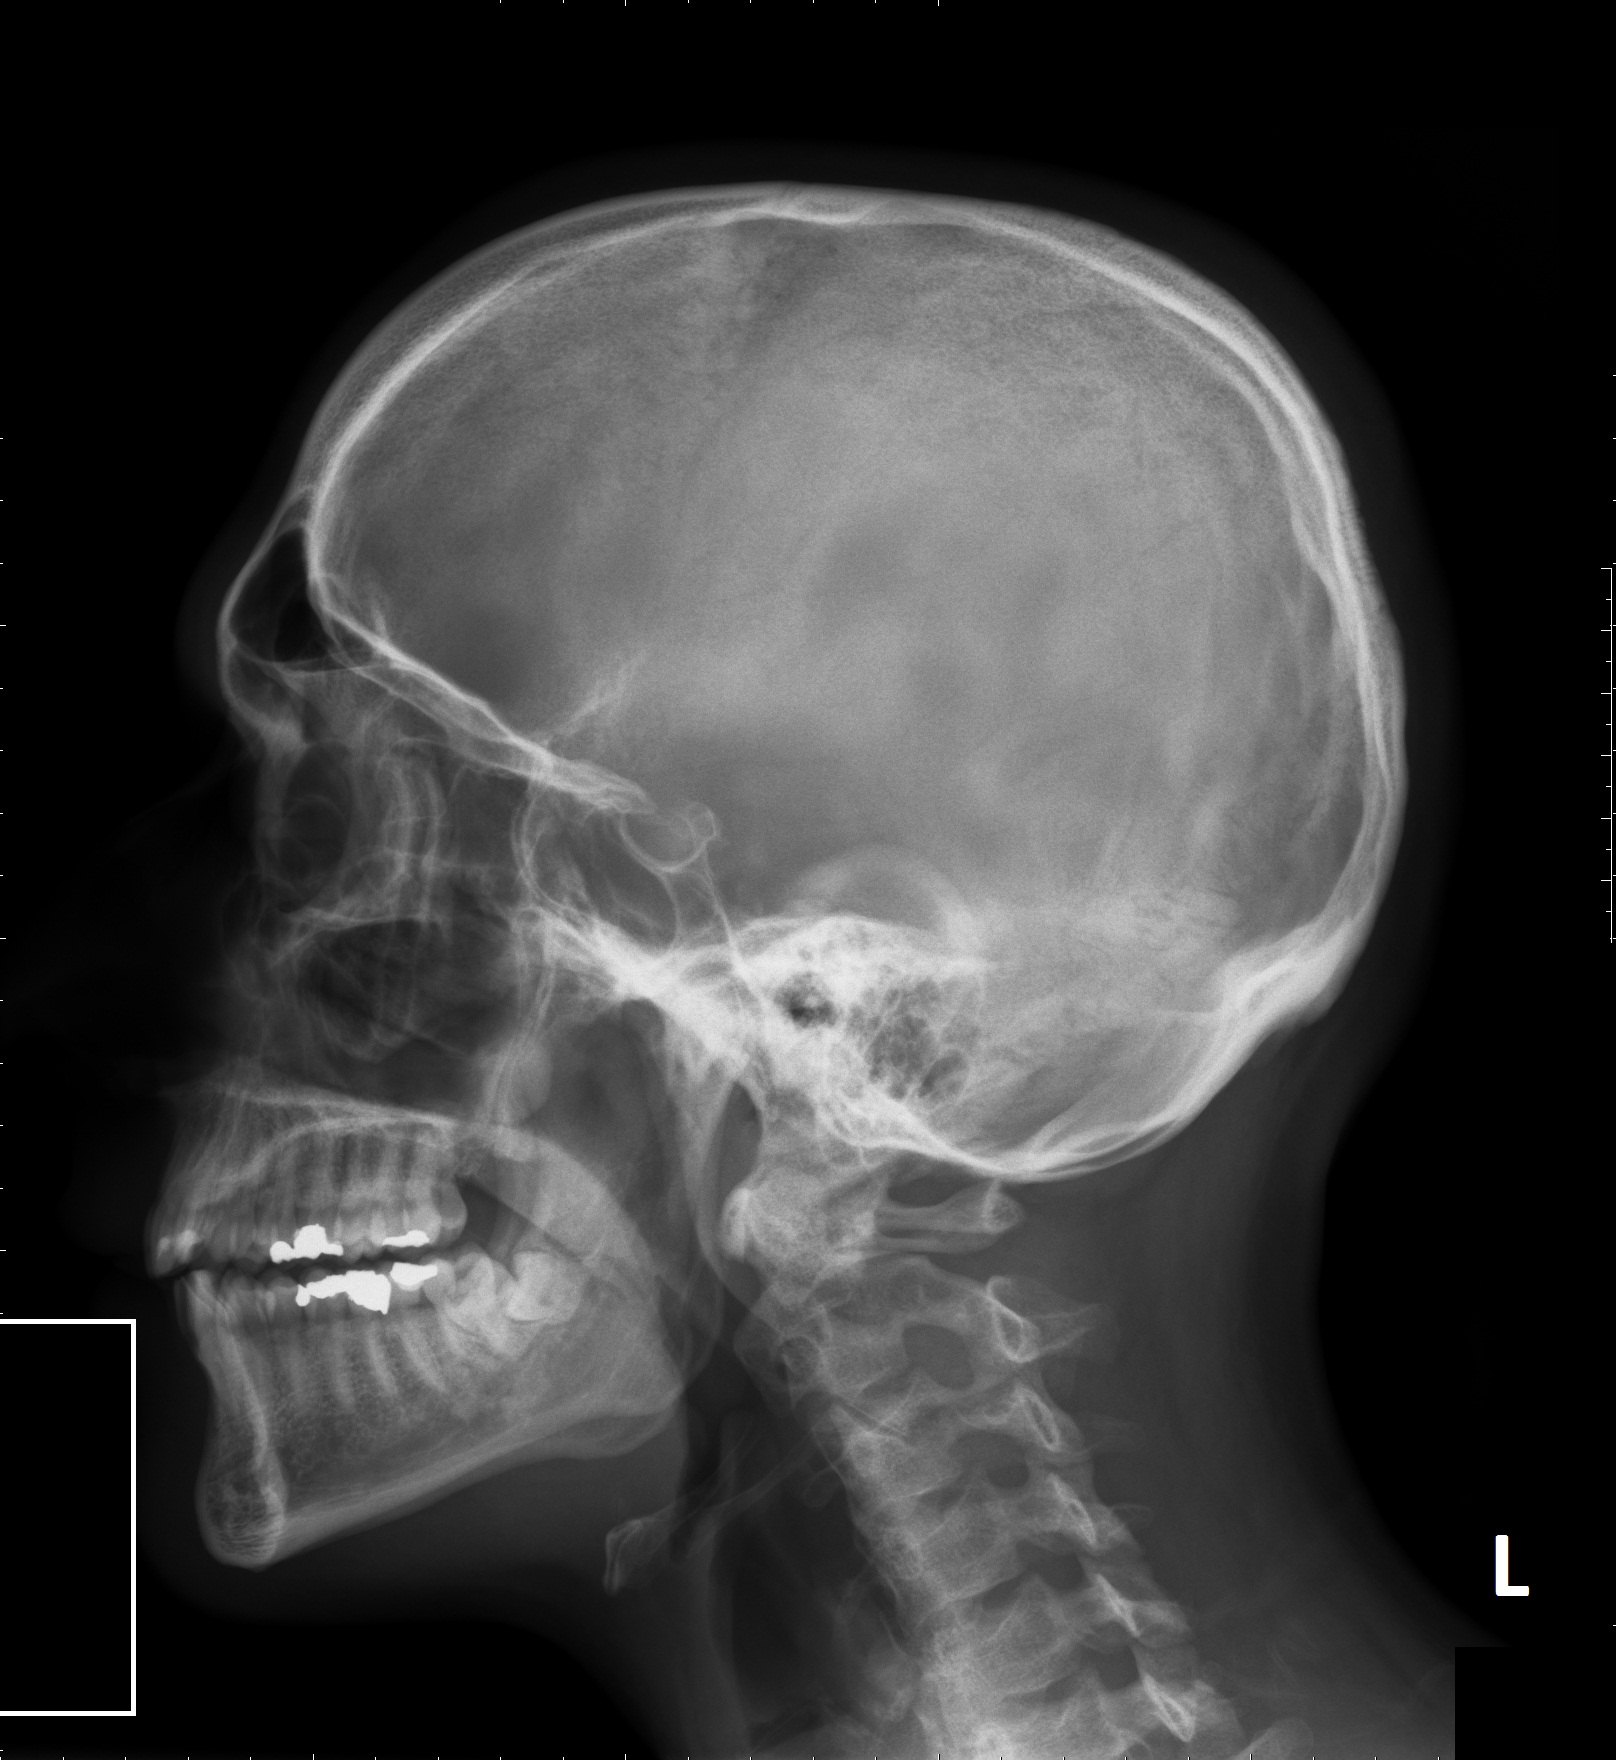
\includegraphics[width=0.4\textwidth]{radiografia}
                        \caption{Una radiografia al cranio - vista laterale.}
                        \label{fig:skull}
                    \end{figure}
                        
                \bigskip
                \par
                    Dalla radiografia in \textit{Figura \ref{fig:skull}}, è possibile distinguere $5$ zone di grigio: Si visualizzano \textit{l'aria} o \textit{tessuti a bassa densità}, di colore grigio molto scuro (tendente al nero); \textit{l'acqua o i tessuti molli}\footnote{Sostanzialmente si vuole definire tutto ciò che non ha la stessa densità dell'osso.}, che si visualizzano con un grigio medio; \textit{il grasso}, evidenziato con un colore grigio scuro; \textit{le ossa}, che presentano una colorazione grigio chiaro; \textit{il campione metallico} (L), di colore praticamente bianco. L’acqua ed i tessuti molli possiedono circa la medesima densità. E' impossibile analizzare il cervello ed evidenziarne un'eventuale patologia, poiché esso è rappresentato come una zona omogeneamente grigia. L'ottenimento di un'immagine del cervello mediante Radiografia Convenzionale divenne una sfida sin dal periodo immediatamente successivo al 1895, anno in cui vennero scoperti i raggi X. Anche il grande scienziato ed inventore Thomas Edison agli inizi del 1900 si cimentò senza successo nell'impresa, a causa delle grosse limitazioni imposte dalla tecnica \cite{thomas-edison-brain}. Il cervello è composto da tessuti molli, racchiusi all’interno di uno scheletro denso che impedisce alla maggior parte della radiazione di penetrarli. Fluttua a bagno in un liquido chiamato \textit{fluido cerebrospinale\footnote{Liquido che fornisce nutrienti ed agisce come cuscino al fine di proteggere la materia grigia stessa}} il che rende ancor più ardua l'impresa. Questo tipo di analisi, si scoprì, essere tecnologicamente inaccessibile alla Radiografia Convenzionale.
                
                \bigskip 
                \par
                    Un radiogramma\footnote{Immagine ottenuta mediante radiografia.} impone diversi limiti diagnostici. Il \textit{problema delle ombre} è una diretta conseguenza del fatto che le complesse strutture tridimensionali del corpo umano, nella radiografia, vengono impresse su lastra bidimensionale. Un tumore, ad esempio, se celato da una struttura ad alta densità come le costole, può passare completamente inosservato alla diagnosi. La lastra radiografica inoltre risulta un mezzo intrinsecamente inadeguato per registrare le differenze di intensità dovute all'attenuazione dei raggi X durante il passaggio attraverso il corpo, non consentendo la distinzione tra i diversi tessuti molli.
                
                \bigskip            
                \par
                    La reale limitazione, nella Radiografia Convenzionale, è l'immensa perdita di informazione riscontrata in fase di acquisizione. Il \textit{problema delle ombre} verrà parzialmente risolto con lo sviluppo della Tomografia Convenzionale, l'analisi dei tessuti molli sarà invece possibile solamente con l'avvento della Tomografia Computerizzata (TC), che consentirà l'accurata misurazione dei valori d'assorbimento, riuscendo a distinguere la natura del materiale o del tessuto.
                            
            \subsection{Tomografia Convenzionale}
            \label{sec:TomografiaConvenzionale}
                \par
                    Per \textit{Tomografia Convenzionale} si intende l'ottenimento di un tomogramma\footnote{Immagine ottenuta mediante tomografia.} senza l'ausilio di computazione. Questa tecnica venne completamente rimpiazzata con la Tomografia Computerizzata intorno al 1980.
                
                \bigskip            
                \par
                    I primi studi risalgono al primo ventennio del 1900 e la tomografia convenzionale, curiosamente, venne indipendentemente scoperta più volte da diversi ricercatori sia Europei che Americani senza che questi scambiassero informazioni: all'epoca, i livelli di comunicazione non erano affatto sviluppati. Un pensiero espresso da Alessandro Vallebona, uno dei cinque grandi pionieri di questa metodologia, era il seguente: \textit{“quando un settore della scienza e della tecnica è maturo per progredire, per fare un passo avanti, il progresso avviene, a volte contemporaneamente oppure a breve distanza di tempo, promosso da persone diverse, anche in Paesi diversi”} \cite{vallebona-pensiero}.
                    Non è infatti difficile recuperare manoscritti nei quali si rivendicano la paternità dell'opera e violazioni d'utilizzo dei brevetti\cite{vallebona-difesa}. Queste ricerche produssero differenti nomenclature, generando molta confusione riguardo l'oggetto di studio. Solamente nel 1962, durante la \textit{International Commission of Radiologic Units and Measurements} (ICRU), venne selezionata la nomenclatura “\textit{Tomografia}”, che venne presto adottata ovunque nel Mondo.
                            
                \bigskip
                \par
                    Il problema delle ombre stimolò la ricerca. Il metodo più convincente per la risoluzione risultò la stratificazione dei tessuti del corpo. In questo modo, utilizzando la geometria proiettiva, il problema poteva essere parzialmente superato, nonostante gli elevati livelli di radiazione richiesti dalla procedura. Per poter eseguire la Tomografia Convenzionale senza computazione, in un puro sistema meccanico, due dei tre elementi (tubo, paziente e lastra) dovevano necessariamente muoversi in modo sincrono durante l’esposizione alla radiazione.  In questo caso il corpo veniva mantenuto fermo, mentre tubo e lastra si muovevano in modo sincrono ed opposto. Solamente circa 1/10 della lunghezza del fascio che attraversava il corpo intersecava effettivamente il piano di interesse, i restanti 9/10 attraversavano il corpo collezionando informazione inutile, non voluta. Questa è la motivazione per cui, in questi tomogrammi, era facile riscontrare artefatti \cite{hounsfield-nobel-lecture}.
                
                \bigskip
                \par
                    I primi pionieri di questa tecnica furono André Edmund Marie Bocage, Alessandro Vallebona, Ziedses des Plantes, Gustav Grossmann e Jean Kieffer. Bocage nel 1922 ottenne il primo brevetto; Vallebona realizzò diversi prototipi e contribuì alla letteratura con ben 370 pubblicazioni nelle scienze radiologiche\cite{vallebona-ricordo}; des Plantes è ritenuto il pioniere della sperimentazione; Grossmann contribuì all’analisi matematica del metodo e rese più snelli i progetti preesistenti; Kieffer fu il primo pioniere Americano, diede una descrizione esaustiva del suo dispositivo e della matematica del sistema. I prototipi creati vennero per lo più utilizzati a scopi di ricerca, l'utilizzo, se a fine clinico, non era affatto confortevole.
                
                \bigskip
                \par
                    Lo sviluppo del primo dispositivo clinico, il Polytome, venne sviluppato a Parigi nel 1950. Le immagini ricavate da questo dispositivo stimolarono le ricerche in ambito clinico, inizialmente dagli Europei e successivamente dagli Americani (anni ‘60).
                    Le applicazioni più frequenti, riguardavano quelle parti del corpo in cui poteva essere presente un alto livello di contrasto, come il cranio. Le immagini sezionali permettevano l’esplorazione dell’intricata rete ossea, tra cui i seni paranasali, la sella turcica\footnote{La sella turcica o sella turca costituisce la faccia superiore del corpo dell'osso sfenoide, un osso impari e mediano del neurocranio.} ed altre aree completamente inaccessibili alla Radiografia Convenzionale. Comparirono successivamente al Polytome diversi nuovi dispositivi che evidenziarono la necessità di ottenere un efficace imaging sezionale \cite{conventional-tomography}.
                
                \bigskip
                \par
                    Si ricorda che la Tomografia Convenzionale non permise l’accesso all’imaging dei tessuti molli, un’immagine sezionale del cervello risulterà quindi possibile solo con l’avvento della Tomografia Computerizzata. Si può storicamente affermare che la Tomografia Convenzionale ha gettato le basi al di sopra delle quali si sono evolute le avanzate tecnologie CT che oggi apprezziamo.
                        
            \subsection{Tomografia Computerizzata}
                \par      
                    La nascita della Tomografia Computerizzata riflette l'evoluzione della tomografia classica. Il pensiero di Vallebona, citato in Sezione \ref{sec:TomografiaConvenzionale}, ha validità anche in questo caso: tre ricercatori, Allan McLeod Cormack, William H. Oldendorf e Godfrey N. Hounsfield, indipendentemente, svilupparono i principi base della TC intorno al 1960. Cormack ed Hounsfield ricevettero il Premio Nobel nel 1979, Oldendorf fu invece vittima di una controversia \cite{nobel-debate} e non venne premiato. 
                    Sia Cormack che Oldendorf ottennero prototipi funzionanti, ma l'ingegnere britannico Sir Godfrey N. Hounsfield fu l'unico in grado di ottenere diverse realizzazioni commerciali di successo.
                
                \bigskip
                \par
                    Hounsfield lavorò dal 1951 per la EMI Ltd di Londra, periodo nel quale si interessò particolarmente ai computer e contribuì alla costruzione del primo computer a transistor in assoluto assemblato in Gran Bretagna \cite{hounsfield-autobiografia}. Successivamente, negli anni '60, egli concepì l’idea della Tomografia Computerizzata ed iniziò le prime sperimentazioni.
                            
                    \begin{figure}[h]
                        \centering
                        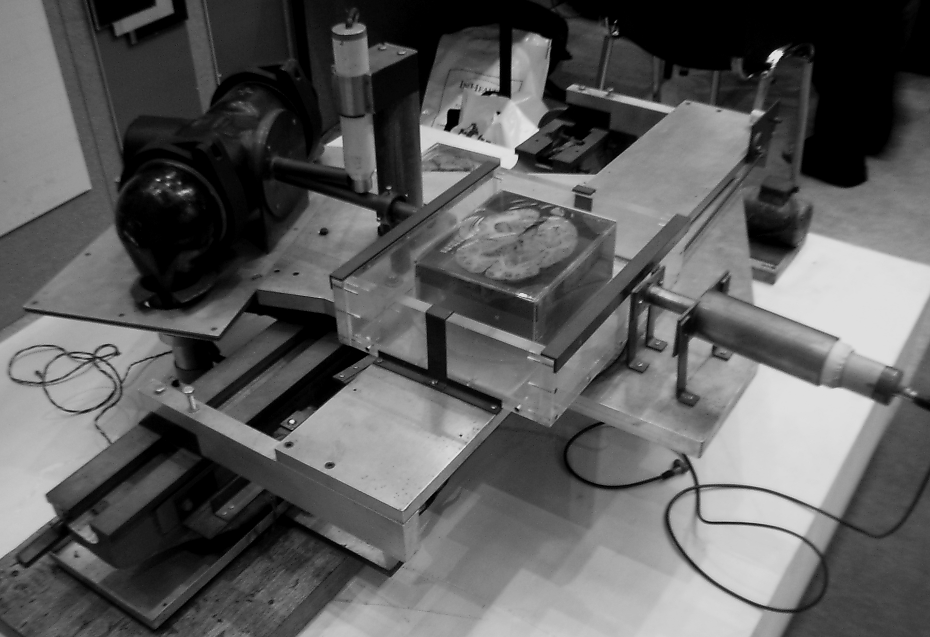
\includegraphics[width=0.5\textwidth]{hounsfield_prototype2}
                        \caption{Il secondo prototipo di Hounsfield. Architettura rotazionale-traslazionale, accompagnata ad un generatore di Raggi X, visibile nel lato sinistro dell'immagine.}
                        \label{fig:second-prototype}
                    \end{figure}
                            
                    Il primo prototipo era composto da una scatola di piombo con un piccolo foro posto nella parte anteriore, all’interno della quale era presente un materiale radioattivo, l’Americium, capace di fornire una fonte costante, non particolarmente intensa, di raggi gamma. La radiazione fuoriusciva dal foro in un singolo fascio collimato a configurazione pencil-beam. Il piatto, sul quale venivano posizionati degli oggetti test (fantocci), veniva traslato orizzontalmente per permettere al singolo fascio di poter raggiungere tutti gli oggetti. Al termine della traslazione, il piatto veniva fatto roteare di $1\degree$, ed il procedimento veniva ripetuto fino all'ottenimento di 180 proiezioni. I livelli d'attenuazione erano letti dal singolo detector opposto alla sorgente. Il processo di scansione durava ben nove giorni, la ricostruzione computerizzata degli oggetti richiedeva più di due ore di processamento. Questo fu un risultato molto importante, poiché dimostrò che la Tomografia Computerizzata era tecnologicamente e fisicamente possibile. Il secondo prototipo di Hounsfield, di medesima geometria ma avente un generatore di Raggi X al posto dell'Americium, è visibile in \textit{Figura \ref{fig:second-prototype}}.
                
                \bigskip
                \par
                    Hounsfield ed i suoi collaboratori, mantenendo la stessa geometria a rotazione-traslazione, continuarono la fase di prototipazione diminuendo via via le tempistiche di acquisizione. Si resero presto conto che l'avanzamento tecnologico avrebbe permesso l'analisi dei tessuti molli, ma non furono ancora certi che questo avrebbe permesso la localizzazione spaziale dei tumori. A verifica di ciò venne creato il primo dispositivo ad utilizzo clinico, molto più veloce e sofisticato rispetto ai prototipi precedenti, dedicato alla sola analisi del cranio, che doveva rimanere estremamente fermo durante l'acquisizione. Nel 1972 la prima paziente in assoluto fu una donna, il cui cervello si pensava presentasse anomalie. La prima immagine rivelò in chiaro ed inconfondibile dettaglio una cisti circolare nera situata nel lobo frontale della paziente, che fu successivamente operata con successo \cite{scanner-story}. Dopo aver analizzato molti altri pazienti divenne inconfutabile il fatto che la macchina fosse perfettamente in grado di effettuare l'analisi dei tessuti molli e di praticare la distinzione tra tessuti sani e malati \cite{hounsfield-nobel-lecture}.
                    
                \bigskip
                \par
                    Per la prima volta nella storia, i limiti imposti dalla Radiografia Convenzionale risultarono completamente superati e si aprì la strada ad una rapida innovazione che coinvolse la riduzione dei tempi di esposizione e l'analisi di tutte le parti del corpo. Il team coordinato da Hounsfield già qualche anno dopo, riuscì a costruire macchinari sempre più complessi, con un tempo di acquisizione prossimo ai tre secondi.
                            
            \subsection{Evoluzione generazionale}
                \par
                    Per evoluzione generazionale si intende la sequenza temporale nel quale un particolare tipo di CT scanner, avente una ben precisa disposizione dei componenti e specifiche caratteristiche nei movimenti meccanici di base, è stato introdotto nel mercato. Va precisato che, al crescere del numero di generazione, non crescono necessariamente le performance del sistema \cite{generazionale}.
                        
                \bigskip
                \par
                    \textbf{Scanner di prima generazione.} La sorgente veniva collimata in un raggio pencil-beam direzionato ad un singolo detector allineato alla sorgente e posizionato all’altro lato dell'oggetto in analisi. Una singola proiezione veniva ottenuta muovendo il tubo sorgente ed il detector in una traslazione sincrona. Per poter ottenere la successiva proiezione, l'apparato di acquisizione ruotava di $1\degree$ e veniva traslata nella direzione opposta. Questo processo doveva essere ripetuto fino all’ottenimento di 180 proiezioni. Le prime versioni richiedevano circa 4 o 5 minuti per poter portare a termine la scansione, ed erano limitate a quelle parti del corpo dove il movimento del paziente poteva essere controllato (cranio). Questa particolare configurazione viene anche detta "\textit{parallel-beam}".
                            
                \bigskip
                \par
                    \textbf{Scanner di seconda generazione.} Aggiungendo multipli detector disposti circolarmente, diverse proiezioni potevano essere ottenute in una singola traslazione. Uno dei primi prototipi, che presentava 3 detector con displacement di $1\degree$, poteva effettuare 60 traslazioni anziché 180. Questo era possibile poiché ciascun detector vedeva la sorgente ad un angolo differente, ottenendo in una singola traslazione ben 3 proiezioni. Il sistema, una volta terminata la traslazione, poteva roteare di $3\degree$  ed ottenere la nuova proiezione. I tempi di scansione venivano quindi ridotti di un terzo. 
                        
                \bigskip
                \par
                    \textbf{Scanner di terza generazione.} In questi scanner, la sorgente è collimata in una struttura a ventaglio (fan-beam) diretta verso i detector disposti ad arco. Durante la scansione, il tubo e l’array di detector ruotano lungo il paziente e differenti proiezioni vengono ottenute durante la rotazione facendo pulsare la sorgente a raggi X oppure campionando i detector ad una frequenza elevata. Il sistema puramente rotazionale ha permesso l’accesso a sorgenti a più elevata potenza, permettendo una notevole riduzione dei tempi d’acquisizione. La divergenza dei raggi, richiede qualche modifica all’interno degli algoritmi di ricostruzione. Tutti gli scanner CT odierni sono basati su modifiche di questo design. 
                            
                \bigskip
                \par
                    \textbf{Scanner di quarta generazione.} Questo particolare design si evolse parallelamente alla terza generazione. In questo caso, venne fatta roteare solo la sorgente mantenendo fisso un intero anello composto da detector. Inizialmente questi dispositivi possedevano 600 detector, successivamente arrivarono fino a 4800, con tempi di acquisizione comparabili agli scanner di terza generazione. Questo design tuttavia presentò diverse limitazioni, quali l’inefficiente utilizzo dei detector (meno di 1/4 venne effettivamente utilizzato ad ogni istante della scansione) ed una maggior suscettibilità alla presenza di artefatti (dovuti allo scattering\footnote{Deflessione dei raggi X dovuta collisione con altri raggi X.}). Per queste ragioni questi scanner non vennero più prodotti..
                            
        \section{Moderne Architetture X-Ray CT}
            \subsection{A Spirale}
                \par
                    Nel 1990, lo sviluppo di questa architettura, (evolutasi dalla geometria Fan-Beam, $3\degree$ Generazione) fu una vera rivoluzione nell'acquisizione CT. Per la prima volta nella storia fu possibile ottenere una scansione tridimensionale dell'intero corpo del paziente con un unica trattenuta di respiro.
                    La tecnica consiste in un'acquisizione continua: mentre sorgente e detector ruotano continuamente, il lettino del paziente viene fatto traslare orizzontalmente all'interno dell'apparato di acquisizione. Questa tecnologia richiese tre avanzamenti tecnologici: la Slip Ring Technology, sorgenti a Raggi X ad elevata intensità ed algoritmi di interpolazione che gestiscano le proiezioni non complanari.
                    
                    \begin{figure}[h]
                        \centering
                        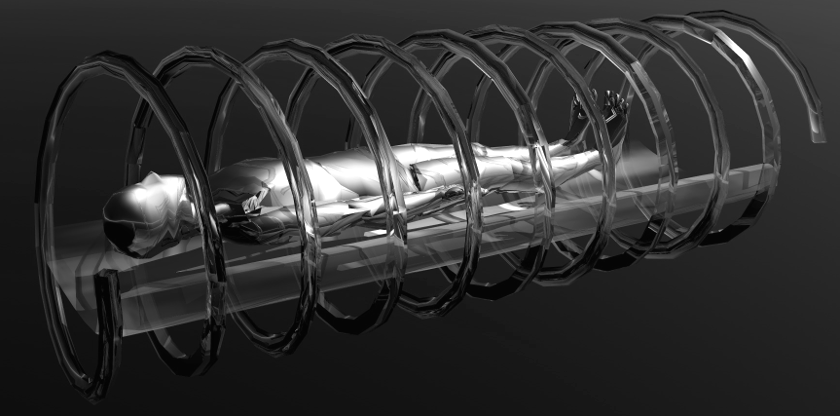
\includegraphics[width=0.6\textwidth]{helical}
                        \caption{Rappresentazione artistica di un'architettura a spirale.}
                        \label{fig:spirale}
                    \end{figure}
                    
                    \bigskip
                    \textbf{Slip Ring Technology.} E' un dispositivo elettromeccanico ad anelli conduttori che trasmettono energia elettrica lungo un frame in movimento. Gli Slip Ring consentono anche lo scambio di informazioni con la parte stazionaria. Questo avanzamento tecnologico consente una continua rotazione dell'apparato di acquisizione senza preoccuparsi dell'avvolgimento dei cavi di sistema.
                    
                    \bigskip
                    \textbf{Sorgenti ad alta energia.} La Slip Ring Technology fu sviluppata al fine di ridurre i tempi di acquisizione, ma una riduzione dei tempi richiese generatori a raggi X a maggiore energia. Una maggiore energia richiede anche una maggior dissipazione di calore. Tutti questi problemi sono stati brillantemente superati, gli apparati a spirale odierni possono effettuare scansioni brevi e ad alta energia riuscendo nel contempo a dissipare l'elevato calore generato.
                    
                    \bigskip
                    \textbf{Algoritmi di Interpolazione.} Un sistema di acquisizione in continuo movimento genera proiezioni che non giacciono su un singolo piano. Ciò significa che gli algoritmi di ricostruzione convenzionali non funzionano correttamente. Il Professor Willi Kallendar ha elaborato un metodo attraverso il quale è possibile generare le proiezioni in un singolo piano, in questo modo algoritmi convenzionali, come FBP, possono essere applicati. 
                    
            \subsection{Cone Beam CT}
                \label{sec:cone-beam}
                \par
                    L'architettura Cone Beam, abbreviata CBCT, prevede l'utilizzo di un detector bidimensionale ed una sorgente che consente la distribuzione del fascio a raggi X a forma conica o piramidale. Fu sviluppato a partire dal 1980 ma il vero potenziale venne apprezzato grazie al lavoro di ricercatori Veronesi che proposero l'utilizzo CBCT in ambito dento-maxillo-facciale\footnote{Imaging di bocca, mascella, mandibola, viso e collo.}. Questa tecnologia trova applicazioni anche nelle procedure angiografiche\footnote{Rappresentazione a scopo diagnostico dei vasi sanguigni o linfatici del corpo umano}, nella radiologia interventistica, radioterapia guidata (IGRT)\footnote{La radioterapia guidata permette di monitorare la reale posizione del volume bersaglio immediatamente prima del trattamento mediante radiazione.}, nella mammografia ed alcuni utilizzi in ambito osteoarticolare e veterinario.
                
                \bigskip
                \par
                    L'apparato di acquisizione compie un giro di $360\degree$ intorno all'oggetto in esame. L'utilizzo di un fascio di tale geometria permette ad ogni esposizione (continua o pulsata) di coprire l'intero campo di vista in un unico giro, anziché effettuare più giri a spirale. Questo consente un abbassamento dei tempi di acquisizione, paragonabili a quelli di una radiografia panoramica.
                                   
                    \begin{figure}[h]
                        \centering
                        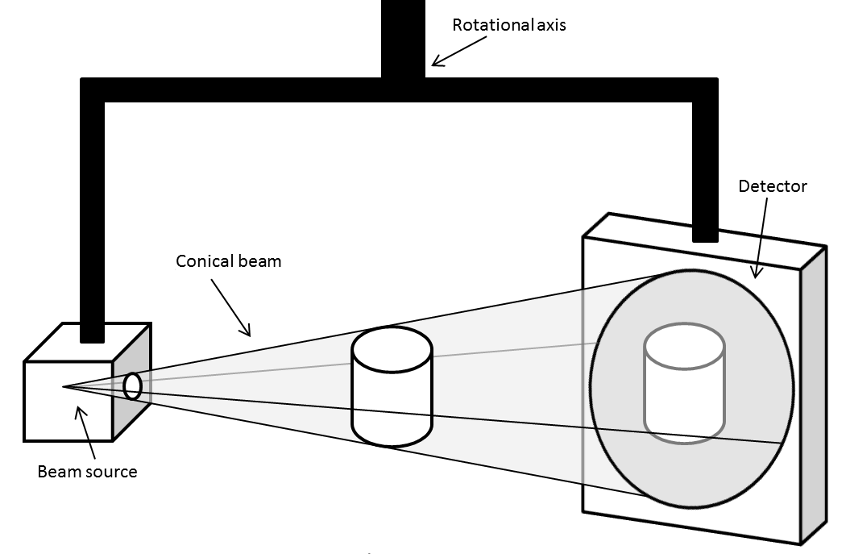
\includegraphics[width=0.55\textwidth]{cone_beam}
                        \caption{Rappresentazione schematica architettura CBCT.}
                        \label{fig:cbct}
                    \end{figure}
                    
                \par
                    Gli algoritmi di ricostruzione risultano molto più complessi rispetto alle ricostruzioni da proiezioni bidimensionali in quanto non esiste un equivalente del "teorema della proiezione" \cite{zeng}.
                    Il primo e più popolare algoritmo di ricostruzione FDK, che prende nome dai ricercatori Feldkamp, Davis e Kress, fornisce solamente ricostruzioni approssimate. Le ricostruzioni contengono artefatti in quelle regioni lontane dal piano orbitale, in quanto il quantitativo di dati selezionati risulta inferiore.
                    Questo algoritmo non è nient'altro che una versione dell'algoritmo di Retroproiezione Filtrata FBP modificato per un set di proiezioni bidimensionale.   
                                            
        \section{Principi di Funzionamento CT}
            \par
                Lo scopo della Tomografia è quello di determinare le strutture interne di un oggetto non trasparente inviando verso questo dei segnali sotto forma di onde/particelle. Possono essere utilizzate onde elettromagnetiche di diversa frequenza ed onde acustiche. La ricostruzione CT è intrinsecamente un problema inverso.
                Il matematico Mark Kac espose chiaramente il concetto di problema inverso nella nota pubblicazione "\textit{Can one hear the shape of the drum?}" \cite{mark-kac}, nel quale essenzialmente si cercò una risposta alla domanda: "E' possibile determinare la forma di una membrana oscillante ascoltando esclusivamente le tonalità prodotte da questa?" Il problema affrontato nella CT è analogo.
            
            \bigskip
            \par
                Johann Radon, matematico Austriaco, pubblicò nel 1917 il suo lavoro relativo alla "Trasformata di Radon". Questo dimostra matematicamente che se gli integrali di linea di una particolare proprietà dell'oggetto in esame, come la densità, possono essere conosciuti per tutte le linee che intersecano una slice di un corpo, complanari alla slice stessa, allora la densità può essere ricostruita esattamente \cite{history-radiology}. Nella pratica l'antitrasformata di Radon, la procedura che permetterebbe la ricostruzione dei livelli di densità, risulta particolarmente instabile. Per questo, negli algoritmi, si utilizzano versioni discretizzate e stabilizzate.
                
            \subsection{Proiezione}
                \par
                    La fase di Proiezione rappresenta la fase di acquisizione, nella quale il detector rileva l'attenuazione del fascio dovuta ai livelli di densità del corpo incontrato.
                \par
                    Matematicamente, nel caso discreto, la fase di proiezione può essere vista in forma matriciale:
                    \begin{equation}
                        y = Ax
                    \end{equation}
                    $A$ rappresenta la matrice di sistema, il modello utilizzato per la Forward Projection, anche detto operatore di proiezione. Il vettore $x$ rappresenta il volume da sottoporre a scansione ed il vettore
                    $y$ rappresenta il set di proiezioni.
                
                \bigskip
                \par
                    Nel caso continuo, se l'oggetto in esame viene rappresentato come una generica funzione densità $f(x,y)$, la Trasformata di Radon a raggi paralleli descrive la procedura di Proiezione in un caso continuo:
                
                    \begin{equation} \label{eq:radon-fwd}
                        p(s,\theta) = \int_{-\infty}^{\infty} \int_{-\infty}^{\infty} f(x,y) \delta(x \cos \theta + y \sin \theta -s) dx dy 
                    \end{equation}
                    
                    Il parametro della funzione $\delta$ assume valore nullo se e solo se il punto $(x,y)$ viene raggiunto dal fascio, in questo caso il contributo $f(x,y)$ viene sommato. Nel caso in cui il punto non sia raggiunto dal fascio, la funzione $\delta$ assume il valore $0$ annullando il contributo di $f$. La funzione $\delta$ è la funzione \textit{delta di Dirac}, dipendente da un parametro reale, così definita:
                    \begin{equation}
                        \delta(x) = \begin{cases} +\infty, & x = 0 \\ 0, & x \ne 0 \end{cases}
                    \end{equation}
                    
                    Ed è inoltre costretta a soddisfare la seguente proprietà:
                    \begin{equation}
                        \int_{-\infty}^\infty \delta(x) \, dx = 1.
                    \end{equation}
            
            \subsection{Normalizzazione delle Proiezioni}
                \label{sec:normalizzazione}
                \par
                    L'intensità dei pixel componenti una proiezione, diretto risultato d'acquisizione da parte del detector, è direttamente proporzionale all'intensità della sorgente. Gli algoritmi di ricostruzione richiedono, per ogni proiezione, l'informazione relativa alla somma dei coefficienti di attenuazione lineare degli $n$ voxel\footnote{Il voxel è un elemento di volume che rappresenta l'informazione in uno spazio tridimensionale, analogamente al pixel che rappresenta informazioni relative ad un'immagine bidimensionale.} dell'oggetto attraversati, informazione indipendente dall'intensità del fascio sorgente. La \textit{Normalizzazione dello Stack} non è altro che il processo di ottenimento della somma dei coefficienti di attenuazione a partire dalla rilevazione del detector.
              
                    \begin{figure}[h]
                        \centering
                        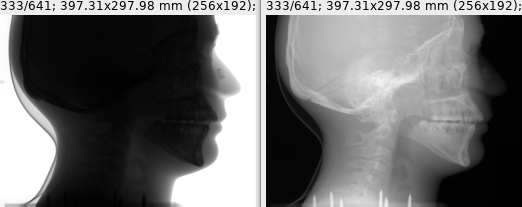
\includegraphics[width=0.6\textwidth]{normalization}
                        \caption{Effetti della procedura di normalizzazione. Immagine a sinistra: non normalizzata. Immagine a destra: normalizzata.}
                        \label{fig:skull-phantom}
                    \end{figure}
                    
                    Le proiezioni, $p(s,\theta)$ (acquisite dal detector) registrano l'intensità attenuata I, la quale è governata dalla legge di Lambert-Beer \cite{lambert-beer} nella forma:
                    
                    \begin{equation} \label{eq:lambert-beer}
                        I = Io \cdot e^{- (\mu1 + \mu2 + ...  + \mu n)}
                    \end{equation}
                    
                    $I$ è l'intensità rilevata dal detector, $\mu_i$ sono i coefficienti di attenuazione lineare appartenenti ad $n$ voxel di larghezza unitaria. Avendo a disposizione l'intensità della sorgente $Io$, è possibile ottenere la somma dei coefficienti di attenuazione lineare manipolando algebricamente (\ref{eq:lambert-beer}):
                        
                    \begin{equation} \label{eq:normalization}
                        (\mu1 + \mu2 + ... + \mu n) = - \log_e{(I/Io)}
                    \end{equation}
                    
                    L'intensità $Io$ dev'essere salvata per ciascuno step angolare $\theta_i$ ponendo, ad esempio, un sensore di rilevazione davanti alla sorgente. Esiste la possibilità, in certe condizioni, di poter stimare $Io$, analizzando quelle zone del fascio rilevate del detector non attenuate dal corpo.
            
            \subsection{Retroproiezione}
                \par
                    Nel caso discreto la retroproiezione può essere espressa in forma matriciale:
                    
                    \begin{equation}
                        \bar{x} = A^\top y
                    \end{equation}
                    
                    La Retroproiezione non permette l'ottenimento del volume originale: $x$ e $\bar{x}$ sono strettamente correlati ma non rappresentano la medesima informazione. $\bar{x}$ è in realtà un'immagine affetta da rumore, che dev'essere eliminato sfruttando particolari tipologie di filtri.
                
                \bigskip
                \par
                    Nel caso continuo, l'immagine retroproiettata $b(x,y)$ può essere ricavata da $p(s,\theta)$ come segue:
                    \begin{equation}
                        b(x,y) = \frac{1}{2} \int_{0}^{2\pi} p(x \cos \theta + y \sin \theta , \theta ) d\theta
                    \end{equation}
                
                \bigskip
                               
            \subsection{Trasformata di Fourier}
                \par
                    Il concetto della trasformata di Fourier è basato sul fatto che è possibile costruire una funzione $p(s)$ come somma pesata di una serie di termini seno e coseno a differenti frequenze, $\nu$, utilizzando una funzione peso $P(\nu)$.
                    
                \bigskip
                \par
                    $P(w)$ per ciascuna frequenza $w$ viene chiamata Trasformata di Fourier di $p(s)$. Uno può facilmente utilizzare formule matematiche per poter ricavare $P(\nu)$ partendo da $p(s)$ e recuperare $p(s)$ da $P(\nu)$. Questo significa che nel caso si conosca una delle due funzioni, si conosce anche l'altra. Utilizzare la Trasformata di Fourier permette di poter comprendere alcune relazioni matematiche nascoste, non facili da osservare senza applicare la Trasformata. E' anche possibile applicare la Trasformata di Fourier ad una funzione con due o più variabili. La Trasformata della funzione $f(x,y)$, viene indicata come $F(\nu_x,\nu_y)$, dove $\nu_x$ rappresenta la frequenza nella direzione $x$ e $\nu_y$ rappresenta la frequenza nella direzione $y$.
                    
            \subsection{Teorema della Proiezione}
                
                \par
                    Il \textit{Teorema della Proiezione}, cuore della Tomografia Computerizzata, afferma che le seguenti procedure sono equivalenti:
        
                    \begin{enumerate}
                        \item Eseguire la Trasformata di Fourier monodimensionale $P(\nu,\theta_i)$ sulla i-esima proiezione $p(s,\theta_i)$
                        \item Selezionare una slice avente la stessa angolazione $\theta_i$ passante per l'origine della Trasformata di Fourier bidimensionale $F(\nu_x,\nu_y)$ eseguita sulla funzione densità $f(x,y)$.  
                    \end{enumerate}
                
                    \begin{figure}[h]
                        \centering
                        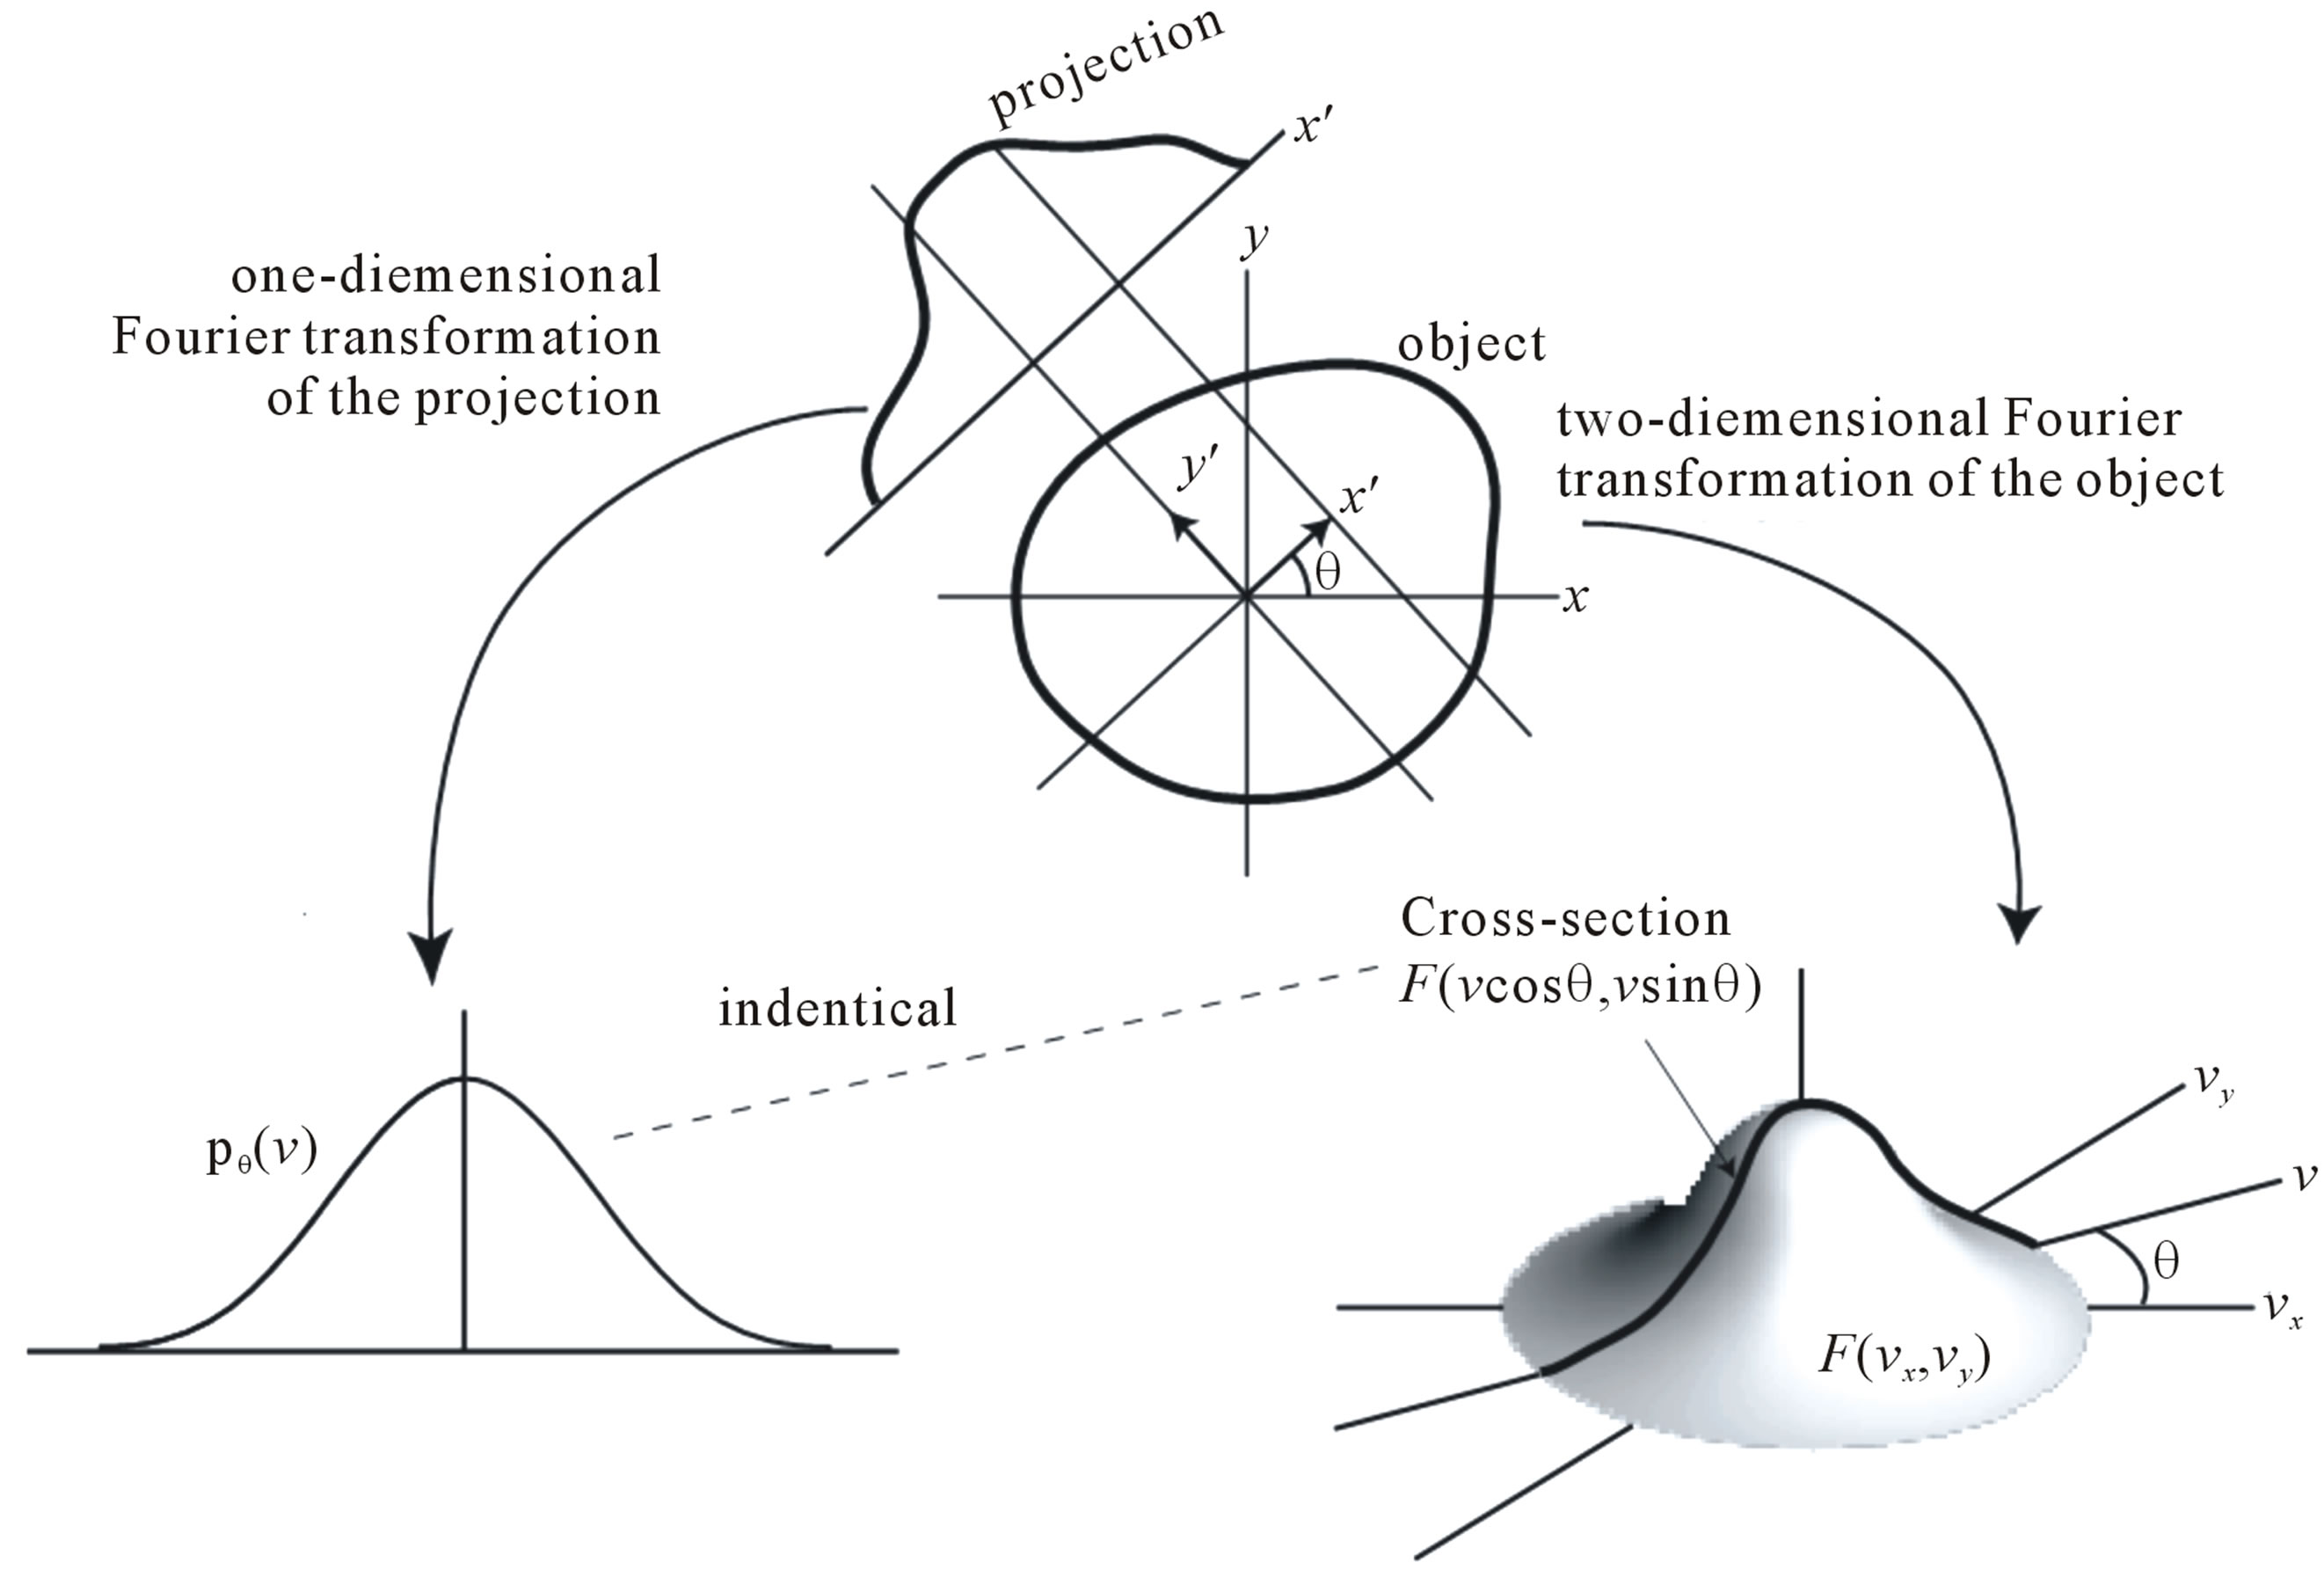
\includegraphics[width=0.6\textwidth]{fourier}
                        \caption{Rappresentazione grafica del Teorema della Proiezione.}
                        \label{fig:itk}        
                    \end{figure}    
            
                \par
                    L'angolazione del detector è rappresentata da $\theta_i$, roteando il detector di almeno $180\degree$ è possibile ottenere l'intera trasformata di Fourier bidimensionale $F(\nu_x,\nu_y)$ senza che questa venga direttamente eseguita sulla funzione densità $f(x,y)$.
                    Una volta ottenuta $F(\nu_x,\nu_y)$, la funzione di densità originale $f(x,y)$ può essere facilmente ottenuta mediante una procedura matematica chiamata antitrasformata di Fourier. Nonostante questa procedura possa teoricamente rimpiazzare la fase di retroproiezione, all'atto pratico ciò non avviene, a causa degli elevati errori di interpolazione che vengono generati dagli algoritmi.
            
            \subsection{Ricostruzione}
                \par
                    In molti algoritmi di ricostruzione si sfrutta la trasformata di Fourier per poter applicare dei filtri in grado di rendere minimo il rumore che differenzia le due immagini $x$ e $\bar{x}$. Ad esempio, l'algoritmo FBP - Filtered Back Projection, uno tra i più conosciuti ed utilizzati, prevede come filtro la moltiplicazione della Trasformata di Fourier monodimensionale $P(\nu,\theta)$ per un filtro detto "a rampa" $|\nu|$. Successivamente, applica l'antitrasformata di Fourier al prodotto $|\nu|P(\nu, \theta)$ e procede alla retroproiezione. In questo caso, avendo applicato il filtro, l'immagine $\bar{x}$ contiene meno rumore ed è comparabile all'originale $x$. Esistono molti algoritmi di ricostruzione e diverse soluzioni riguardo l'applicazione dei filtri. Alcuni algoritmi applicano i filtri senza calcolare la trasformata di Fourier, altri utilizzano altri tipi di trasformazione come quella di Hilbert. 
                \bigskip
                \par
                    Esistono algoritmi di ricostruzione che effettuano procedimenti iterativi, combinando procedure di Simulated Forward e Back Projection. Un algoritmo iterativo FBP, può essere matematicamente espresso come segue \cite{fessler}:
                   
                   \begin{equation}
                        x_{n+1} = x_n + \alpha FBP( y - Ax_n)
                    \end{equation}
                    
                    Le proiezioni iniziali sono date da $y$, $Ax$ è una fase di Proiezione simulata (non si effettua un'acquisizione reale) sfruttando i dati dell'iterazione precedente ed $\alpha$ è una variabile peso. Questi algoritmi richiedono un costo computazionale proporzionale al numero di iterazioni effettuate. Nel caso di una singola iterazione, la complessità è paragonabile a quella dell'algoritmo originale.
                    
        \section{OpenRTK}
            \label{sec:openrtk}
            \par
                Il progetto, rilasciato sotto licenza Apache 2.0, nacque nel Giugno 2010 quando i founder Simon Rit e Gregory Sharp discussero riguardo la scarsità di soluzioni open-source nell'ambito della Cone Beam CT. Infatti, l'unica alternativa presente era una libreria chiamata Plastimatch, la quale poteva già effettuare retroproiezioni filtrate sia su CPU che su GPU, ma l'architettura del software non teneva conto dell'evoluzione verso nuove tipologie di algoritmi iterativi. Decidettero quindi di dar vita ad una nuova piattaforma basata su Insight ToolKit (ITK), una libreria di elaborazione delle immagini già famosa in quegli anni. Gli sviluppi iniziali furono basati su codici preesistenti, la piattaforma permise in breve tempo l'ottenimento di ricostruzioni FBP utilizzando dati provenienti da diversi scanner commerciali CBCT. Questi sviluppi attirarono l'interesse dell'Università Cattolica di Lovanio e dell'azienda Beam Application (IBA). RTK è ora utilizzato negli scanner commerciali di IBA. Al giorno d'oggi questi partner sono riuniti presso l'RTK Consortium.
            
            \bigskip
            \par
                RTK è una libreria scritta in linguaggio C++ ma presenta un'interfaccia di utilizzo per altri linguaggi. SimpleRTK \cite{simplertk-wiki} permette l'utilizzo RTK per i linguaggi C\# e Python, ma sono possibili estensioni anche ad altri linguaggi quali Lua e Java, sfruttando SWIG \cite{swig-website}.  RTK fornisce algoritmi di ricostruzione sia sequenziali (FDK) che iterativi (ADMM, SART, Conjugate Gradient, Iterative FDK, ...), presentando delle varianti degli stessi a seconda delle tipologie di filtering applicate. Sono inoltre presenti delle classi ottimizzate per il calcolo parallelo su architetture CUDA \cite{cuda}. E' possibile consultare l'intera lista delle classi che implementano gli algoritmi di ricostruzione nella documentazione ufficiale \cite{rtk-classi}. 
                Questa descrizione è relativa alla versione di RTK numero 1.3.0, rilasciata il 22/09/2016.
                    
            \subsection{Geometria}
                \label{sec:rtk-geometry}
                \par
                    RTK necessita di informazioni relative alla geometria di acquisizione per poter correttamente ricostruire un set di proiezioni. La classe che gestisce queste informazioni è\textit{ ThreeDCircularProjectionGeometry}, basata nello standard internazionale IEC 61217 che è stato progettato per dispositivi cone-beam su sistemi isocentrici. Il sistema a coordinate fisse di RTK ed il sistema di coordinate fisse dell'IEC 61217 sono esattamente uguali. Il sistema consente anche il salvataggio e la lettura della geometria su file XML.
                
                \bigskip
                \par
                    E' possibile impostare fino a 9 parametri in doppia precisione per ciascuna proiezione, sfruttando il metodo \textit{AddProjection}. Viene impostato il valore di default $0$ per tutti quei parametri non esplicitamente espressi. Di seguito vengono analizzati i 5 parametri fondamentali:
                        
                    \begin{itemize}
                        \item \textbf{SID} - Source to Isocenter\footnote{L’asse centrale del fascio interseca l’asse di rotazione dell'apparato di acquisizione in un punto dello spazio chiamato Isocentro} Distance, espressa in millimetri.
                        \item \textbf{SDD} - Source to Detector Distance, espressa in millimetri.
                        \item \textbf{gantryAngle} - E' l'angolo di rotazione del Gantry\footnote{Asse di rotazione dell'apparato di acquisizione, composto da sorgente e detector allineati.}. Un incremento di questo parametro corrisponde ad una rotazione oraria del Gantry visto dall'Isocentro.
                        \item \textbf{projOffsetX} - Offset nella direzione $x$ dall'origine del detector (proiezione ortogonale dell'isocentro sul detector) all'origine dell'immagine di proiezione \cite{rtk-users-proj-offset}. Espresso in millimetri. 
                        \item \textbf{projOffsetY} - Offset nella direzione $y$, come descritto per projOffsetX. Espresso in millimetri.
                    \end{itemize}
                    
                    Per la descrizione dei rimanenti parametri (outOfPlaneAngle, inPlaneAngle, sourceOffsetX, sourceOffsetY), utilizzabili solamente in particolari geometrie, si rimanda alla documentazione \cite{rtk-geometry}.
                
        \section{SimpleITK}
            \par
                SimpleITK, rilasciato sotto licenza Apache 2.0, fornisce un'interfaccia semplificata del software Insight Toolkit - ITK. Può essere utilizzato per poter eseguire un processing generico su varie tipologie di immagini, ma lo scopo principale del Toolkit è quello di processare immagini a scopo medico. Un errato settaggio delle componenti fondamentali, può produrre risultati inconsistenti. Le immagini a scopo medico, senza alcun tipo di informazione spaziale, non dovrebbero assolutamente essere utilizzate per la diagnosi. In altre parole, le immagini a scopo medico che presentano un'inefficienza riguardo le informazioni spaziali, non sono solamente inutili, ma anche pericolose \cite{itk-doc}. Come per SimpleRTK, SimpleITK permette l'utilizzo di ITK su linguaggi quali Python e Java, sfruttando SWIG. Questa descrizione è relativa alla versione di SimpleITK numero 0.9.0, rilasciata il 14/05/2015.
                
            \subsection{Descrizione delle immagini}
            \label{sec:descrizione-immagini}
                Le componenti fondamentali nella descrizione di un'immagine mediante ITK sono \textit{Spacing}, \textit{Origin}, e \textit{Direction}. Se questi parametri vengono settati correttamente, l'immagine avrà ciascun pixel mappato sullo spazio di coordinate fisiche. Un \textit{pixel} è considerato essere la regione quadrata o rettangolare che ne circonda il suo centro, contenitore di informazione. I pixel possono essere visti come la regione di Voronoi \cite{voronoi} della griglia dell’immagine. L’interpolazione lineare dei valori dell’immagine viene eseguita all’interno della regione di Delaunay \cite{delaunay}, i cui angoli sono il centro del pixel. 
                
                \begin{figure}[h]
                    \centering
                    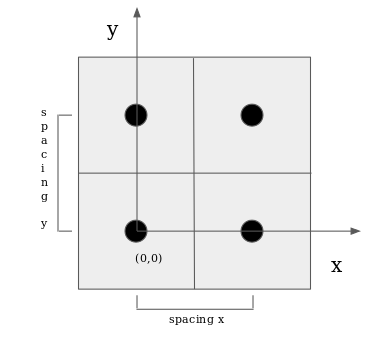
\includegraphics[width=0.5\textwidth]{itk}
                    \caption{Gestione immagini in ITK, configurazione di default.}
                    \label{fig:itk}        
                \end{figure}
                
                \bigskip
                \textbf{Spacing} - Lo Spacing, la distanza fisica tra i centri dei pixel, viene misurato in millimetri. Viene rappresentato come un array fisso le cui dimensioni corrispondono alle dimensioni dell'immagine. Nel caso in cui Spacing non venga impostato, assume di default il valore $1$ in ciascuna componente.
                
                \bigskip
                \textbf{Origin} - Viene gestito vettorialmente, in modo simile allo Spacing. Le coordinate di Origin possono essere assegnate a ciascuna componente. Queste coordinate, di default, corrispondono alla posizione del centro del primo pixel in basso a sinistra dell'immagine rispetto ad un sistema di riferimento fisico, in millimetri. Nel caso in cui Origin non venga impostato, questo assumerà di default il valore $0$ in ciascuna componente. Ad esempio, nel caso in cui si lavori con un'immagine 2D, l'origine del sistema di riferimento fisico giacerà esattamente nel primo pixel in basso a sinistra dell'immagine bidimensionale (Figura \ref{fig:itk}). 
                
                \bigskip
                \textbf{Direction} - Direction rappresenta la relazione d'orientazione tra i pixel ed il sistema di riferimento fisico. Direction è una matrice ortonormale, che descrive la possibile permutazione dei valori dell'immagine e gli aspetti rotazionali che sono necessari al fine di riconciliare correttamente l'organizzazione degli indici dell'immagine con lo spazio fisico. Nel caso in cui Direction non venga impostato, esso è di default una matrice Identità, ciò sta ad indicare che i pixel (voxel) sono perfettamente allineati rispetto al sistema di riferimento fisico.
                
            \subsection{Formati MHA/MHD}
                \label{sec:mha}
                \par
                    I formati MetaImage MHA ed MHD sono file text-based contenenti TAG utilizzati per immagini a scopo medico. Attualmente MetaImage è in grado di supportare una varietà di oggetti quali cubi, sfere, tubi, etc. Questo formato è particolarmente stabile, utilizzato per diversi anni da molti ricercatori all'UNC, Chapel Hill. Occasionalmente vengono introdotte nuove features, ma viene sempre mantenuta la retrocompatibilità con le versioni precedenti. 
                
                \bigskip
                \par
                    Il formato MetaImage prevede alcuni TAG obbligatori, che devono essere inseriti all'inizio del file. Ad eccezione del TAG \textit{ElementDataFile}, posizionato necessariamente come ultimo della lista, l'ordine dei TAG non è rilevante. Il formato MHA prevede che \textit{ElementDataFile} contenga il valore \textit{Local} e che i dati grezzi RAW \cite{raw} siano posizionati nella riga immediatamente successiva alla lista dei TAG. Un file avente estensione MHD, al contrario, prevede che i dati RAW siano collocati in un file esterno e che \textit{ElementDataFile} ne contenga il nome o il percorso. SimpleITK non è fornita di una classe che permette la lettura diretta di un file RAW, per questo motivo il formato MHD risulta particolarmente utile.
                
                \bigskip
                \par
                    I TAG obbligatori sono: NDims, DimSize, ElementType, ElementByteOrderMSB, ed ElementDataFile. I TAG relativi a Spacing, Origin e Direction assumeranno i valori di default precedentemente descritti se non espressamente indicati. Un file MHD si visualizza come in questo esempio:
                    
                    \begin{lstlisting}[language=bash, frame=bt]
NDims = 3
DimSize = 256 250 64
ElementType = MET_FLOAT
ElementByteOrderMSB = True
ElementDataFile = data.raw
                    \end{lstlisting}
                    
                    \begin{itemize}
                        \item \textbf{NDims} Intero che sta ad indicare la dimensione dell'immagine.
                        \item \textbf{DimSize} Array intero, specifica la dimensione in pixel dell'immagine nelle componenti indicate mediante NDims.
                        \item \textbf{ElementType} Specifica il tipo di dato che il sistema andrà a leggere. Può assumere uno tra i valori specificati in \textit{metaTypes.h} reperibile nella documentazione ufficiale \cite{mha-doc}.
                        \item \textbf{ElementByteOrderMSB} Può assumere i valori \textit{True} oppure \textit{False} a seconda dell'architettura del sistema \cite{endianness}.
                        \item \textbf{ElementDataFile} Come già descritto, può assumere il valore \textit{Local} oppure il nome del file RAW esterno a seconda che si stia descrivendo un file MHA oppure un file MHD. Dev'essere posizionato obbligatoriamente come ultimo TAG della lista.
                    \end{itemize}
                    
                    Spacing può essere impostato nelle varie direzioni sfruttando uno dei TAG equivalenti \textit{ElementSpacing} e \textit{ElementSize}. Origin può essere impostato nelle varie direzioni, mediante uno dei tre TAG equivalenti: \textit{Position}, \textit{Offset} ed \textit{Origin}. Direction può essere impostata mediante uno dei tre TAG equivalenti: \textit{Rotation}, \textit{Orientation} e \textit{TransformMatrix}. Ad esempio, nel caso in cui ci si riferisca all'esempio precedente, i TAG per Spacing, Origin e Direction possono essere impostati come segue:
                    
                    \begin{lstlisting}[language=bash, frame=bt]
ElementSpacing = 1.5 1.5 1.5
Position = -10 -10 -10
Rotation = 1 0 0 0 1 0 0 0 1
                    \end{lstlisting}
                    
                    Spacing è stato impostato ad 1.5 millimetri in ogni direzione, Origin è stato impostato a -10 millimetri in ogni direzione e Rotation è stata impostata, come di default, ad una matrice Identità. Il parametro Rotation rispetta il formato MET\textunderscore FLOAT\textunderscore MATRIX, consultabile nella documentazione ufficiale.
                                     
                                              
    \chapter{Sviluppo del Progetto}
        \par
            Nelle seguenti sezioni verrà descritto come ottenere la ricostruzione tomografica di uno Stack di proiezione in formato RAW non normalizzato, avente opportune informazioni associate, sfruttando uno tra gli algoritmi forniti da RTK. Questo coinvolge la conversione dello Stack RAW in formato MHA, la normalizzazione dello Stack MHA e la corretta generazione della geometria di acquisizione in formato XML. 
            
        \bigskip
        \par
            La procedura di compilazione di \textit{RTK}, che coinvolge anche la compilazione di ITK, è stata riscritta in uno script Bash \cite{script-bash} che automatizza completamente le operazioni descritte nel tutorial ufficiale. Sfruttando l'adozione di uno speciale parametro per la compilazione \cite{parallel-j}, è stato possibile ottenere un consistente risparmio in termini di tempo. La community OpenRTK, dopo esserne entrata a conoscenza grazie alla mailing list Rtk-users, ha inserito lo script nel tutorial di installazione ufficiale \cite{wiki-rtk}. La procedura di configurazione ed installazione di \textit{SimpleRTK}, non inserita nello script, è stata eseguita seguendo esattamente le indicazioni fornite dal sito ufficiale \cite{simplertk-install}. SimpleITK è stato aggiunto all'environment locale Python utilizzando il package manager PIP \cite{python-pip}, come descritto nella rispettiva documentazione \cite{simpleitk-install}.

        \section{Stack di proiezione RAW}
            \par
                La Facoltà ha messo a disposizione una decina di Stack di Proiezione in formato RAW (grezzo), acquisiti mediante architettura CBCT. Ciascuno Stack, non normalizzato, era accompagnato da un file CSV e da un file di testo descrittivo. Le informazioni contenute nel file di testo descrittivo, valide per ciascuna proiezione appartenente allo Stack, erano le seguenti:
                    
                \begin{itemize}
                    \item $SID$, $SDD$ - Distanza Sorgente Isocentro e Distanza Sorgente Detector, in millimetri.
                    
                    \item $du$, $dv$ - Larghezza ed altezza di un singolo pixel di una proiezione bidimensionale nel sistema di riferimento $(u,v)$, in millimetri.
                    
                    \item $N_u$, $N_v$ - Numero di pixel componenti una proiezione bidimensionale nel riferimento $(u,v)$.
                    
                    \item \textit{Dimensione dello Stack (X,Y,Z)} - La direzione Z indica il numero di proiezioni bidimensionali appartenenti allo Stack. X ed Y indicano la dimensione proiezioni in pixel ed equivalgono ad $N_u$ ed $N_v$, rispettivamente.
                \end{itemize}
                    
                Il sistema di riferimento $(u,v)$ differisce dal sistema $(x,y)$ di ITK in quanto l'asse $v$ ha direzione opposta rispetto all'asse $y$ e l'origine del sistema di riferimento è situata nel centro del pixel in alto a sinistra dell'immagine (Si confronti Figura \ref{fig:itk} con Figura \ref{fig:uv}).
                    
                \begin{figure}[h]
                    \centering
                    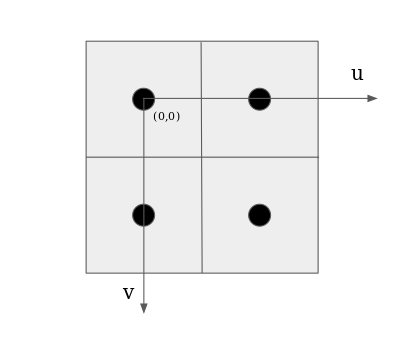
\includegraphics[width=0.55\textwidth]{uv}
                    \caption{Il sistema di riferimento $(u,v)$.}
                    \label{fig:uv}
                \end{figure}
                
                La conversione da coordinate $(u,v)$ a coordinate $(x,y)$ può essere vettorialmente espressa in questo modo:
                \begin{equation} \label{eq:uv-conversion}
                    (x,y) = ( u, N_v - 1 - v )
                \end{equation}
                    
            \bigskip    
            \par
                Il file CSV, conteneva per ciascuna riga informazioni relative alle proiezioni componenti lo Stack. Il numero di righe del file corrispondevano alla dimensione Z dello Stack, quindi, al numero di proiezioni. Ciascuna proiezione veniva associata ad una riga del file: La $1\degree$ proiezione dello Stack era associata alla riga $1$, la $2\degree$ proiezione alla riga $2$ e così via. Ciascuna riga era così composta: 
                    
                \begin{lstlisting}[language=bash, frame=bt] 
+-----------------+-------+--------+--------+----+
| Projection Name | Angle | Niso_u | Niso_v | Io |
+-----------------+-------+--------+--------+----+
                \end{lstlisting}
                    
                \begin{itemize}
                    \item \textit{Projection Name} - E' un dato puramente indicativo. Può essere utilizzato come nomenclatura nel caso in cui lo Stack tridimensionale RAW venga esportato in $n$ file di proiezione bidimensionali.
                        
                    \item \textit{Angle} - E' l'angolo nel quale la proiezione è stata acquisita. Corrisponde a \textit{gantryAngle}, descritto in Sezione \ref{sec:rtk-geometry}.
                        
                    \item \textit{($N_{iso\textunderscore u},N_{iso\textunderscore v}$)} - Posizione dell'origine del detector (proiezione ortogonale dell'isocentro sul detector) nel sistema di riferimento $(u,v)$, in numero di pixel.
                        
                    \item \textit{$Io$} - Intensità della sorgente durante l'acquisizione della proiezione, descritta in Sezione \ref{sec:normalizzazione}.
                \end{itemize}
                
            
        \section{Generazione MHA da Stack RAW}
            \label{sec:conversione}
            \par
                La gestione di un'immagine MHA risulta più semplice, in quanto l'intera informazione (TAG e dati grezzi) è descritta in un singolo file. Si è inizialmente generato un file MHD contenente i TAG obbligatori (Sezione \ref{sec:mha}) e le informazioni relative allo Spacing, come in questo esempio:
                    
                \begin{lstlisting}[language=bash, frame=bt]
NDims = 3
DimSize = 1024 512 200
ElementSpacing = 0.096 0.096 1.8
ElementType = MET_FLOAT
ElementByteOrderMSB = True
ElementDataFile = Contra_40kV_Al_2mm_1024_512_200f.raw
                \end{lstlisting}
                    
                La terza componente di ElementSpacing, $1.8$ millimetri, indica che sono state eseguite 200 proiezioni in un angolo di $360\degree$. Questo non è obbligatorio poiché Spacing si riferisce alla distanza fisica, nella direzione Z, tra i centri dei pixel delle proiezioni bidimensionali all'interno dello Stack. Le informazioni relative ad Origin e Direction non sono state impostate in quanto i valori di default sono adatti allo scopo (Sezione \ref{sec:descrizione-immagini}).
                    
                \bigskip
                \par
                Il file RAW può essere letto mediante SimpleITK, sfruttando il file MHD appena generato: \textit{proj\textunderscore stack.mhd}.
                   
                \begin{lstlisting}[language=python, frame=bt]
>>> import SimpleITK as sitk
>>> image = sitk.ReadImage('proj_stack.mhd')
>>> sitk.WriteImage(image, 'proj_stack.mha')
                \end{lstlisting}
                    
                Il metodo \textit{ReadImage()} legge il file \textit{proj\textunderscore stack.mhd} e restituisce un oggetto Image \cite{itk-image-object}. Il metodo \textit{WriteImage()} \cite{sitk-write-image} scrive su file l'oggetto in formato MHA, nominandolo \textit{proj\textunderscore stack.mha}. 
        
        \section{Lettura informazioni da file CSV}
            \label{sec:lettura-csv}
            
            \par
                Per la gestione delle informazioni appartenenti a ciascuna riga del file CSV è stata creata una Classe Python così definita:
            
                \begin{lstlisting}[language=python, frame=bt]
class Projection(object):
    def __init__(self, name, angle, Niso_u, Niso_v, io):
        self.name = str(name)
        self.angle = float(angle)
        self.Niso_u = float(Niso_u)
        self.Niso_v = float(Niso_v)
        self.io = float(io)
                \end{lstlisting}
            
               Il costruttore della Classe, \textit{\textunderscore \textunderscore init\textunderscore \textunderscore}, riceverà come parametri i contenuti di una riga del file CSV. Per poter acquisire l'intera informazione contenuta nel file, verranno creati $n$ Oggetti Projection, con $n$ corrispondente al numero di righe del file.
            
            \bigskip
            \par
                Si è sfruttato il Python Package \textit{pyexcel} \cite{pyexcel}, che fornisce un'interfaccia API per la lettura e manipolazione di file CSV. La lettura viene gestita attraverso la funzione \textit{get\textunderscore sheet()} che restituisce un'istanza della classe \textit{Sheet} definita all'interno del core \textit{pyexcel}:
                
                \begin{lstlisting}[language=python, frame=bt]
csv = pyexcel.get_sheet(file_name = 'file.csv')
                \end{lstlisting}
            
            \bigskip
            \par
                Un oggetto della classe \textit{Sheet} contiene tutti i dati del file CSV sotto forma di lista bidimensionale \cite{pyexcel-docs}. La prima dimensione consente di accedere ad una singola riga:
                
                \begin{lstlisting}[language=python, frame=bt]
>>>csv[0]
['00000.tiff', 181.79, 128.5, 96.5, 39162]
                \end{lstlisting}
            
                Anche la singola riga è rappresentata come lista, l'accesso ad una singola cella diventa:
                \begin{lstlisting}[language=python, frame=bt]
>>> csv[0][0]
'00000.tiff'
                \end{lstlisting}
            
            \bigskip
            \par
                Sfruttando le proprietà sopra descritte e sfruttando l'iterabilità delle liste fornita da Python \cite{python-list}, si è potuto iterare su tutte le righe del file sfruttando un ciclo FOR:
            
                \begin{lstlisting}[language=python, frame=bt]
proj_obj_list = []
for row in csv:
    proj = Projection(row[0],row[1],row[2],row[3],row[4])
    proj_obj_list.append(proj)
                \end{lstlisting}
            
                Si è creata una lista vuota, \textit{proj\textunderscore obj\textunderscore list}. Grazie al metodo \textit{append} \cite{python-append}, appartenente all'oggetto \textit{list} di Python, è possibile concatenare un'istanza della classe Projection alla lista. Al termine del ciclo, la dimensione della lista coincide con il numero di righe presenti all'interno del file CSV.
            
            \bigskip
            \par
                Questa configurazione, permette un accesso all'informazione facilmente comprensibile. Nel caso in cui si voglia accedere, ad esempio, all'informazione $Io$ della $1\degree$ proiezione, è sufficiente accedere all'omonimo attributo dell'oggetto creato, nella posizione desiderata: 
            
                \begin{lstlisting}[language=python, frame=bt]
>>> proj_obj_list[0].io
39162.0
                \end{lstlisting}
            
               In Python l'indicizzazione delle liste parte dall'indice $0$, dunque la $1\degree$ proiezione dello Stack è identificata dall'indice $0$, la $2\degree$ dall'indice $1$ e così via.
        
        \section{Normalizzazione Stack MHA}
            \label{sec:norm-disp}
            
            \par
                Uno Stack di proiezione, convertito da formato RAW a formato MHA, deve essere normalizzato secondo la procedura descritta in Sezione \ref{sec:normalizzazione} per poter essere correttamente utilizzato dagli algoritmi di ricostruzione forniti da RTK. Ciò richiede l'ottenimento dei valori $Io$, che possono essere recuperati dalla lista \textit{proj\textunderscore obj\textunderscore list} generata a partire dal file CSV associato allo Stack, come descritto in Sezione \ref{sec:lettura-csv}. La lettura dello Stack MHA è invece affidata al metodo \textit{ReadImage()} di SimpleITK, il quale genera un' oggetto Image \cite{sitk-image}:
                
                \begin{lstlisting}[language=python, frame=bt]
stack = sitk.ReadImage(proj_stack.mha)
                \end{lstlisting}
                
                L'oggetto \textit{stack} possiede ora i metodi \textit{GetWidth()}, \textit{GetHeight()} e \textit{GetDepth()}, utili per reperire le informazioni dimensionali dello Stack, precedentemente inserite nella sua creazione (Sezione \ref{sec:conversione}):
                \begin{lstlisting}[language=python, frame=bt]
width = stack.GetWidth()
height = stack.GetHeight()
depth = stack.GetDepth()
                \end{lstlisting} 
                
                E' stata poi creata una lista vuota, che conterrà le singole proiezioni estratte e normalizzate (oggetti Image bidimensionali):
                \begin{lstlisting}[language=python, frame=bt]
norm_proj_list = []
                \end{lstlisting}
                
                Si è successivamente configurato un ciclo FOR, iterante sulla profondità \textit{depth}, corrispondente al numero di proiezioni presenti nello Stack:
                \begin{lstlisting}[language=python, frame=bt]
for zslice in range(0, depth):
                \end{lstlisting} 

                La variabile \textit{zslice} assume i valori interi $0 \leq zslice < depth$ in quanto la funzione built-in \textit{range()} \cite{python-range} di Python genera una sequenza di interi \textit{iterable} \cite{python-iterable} appartenenti al dominio appena indicato. La procedura di normalizzazione avviene all'interno di questo ciclo, dove si susseguono ripetutamente le seguenti fasi, fino all'esaurimento dello Stack:
                
                \begin{enumerate}
                    \item \textbf{Estrazione di una singola Proiezione}. Viene affidata alla Classe \textit{ExtractImageFilter} \cite{sitk-estractor} di SimpleITK. Questa permette il collasso delle dimensioni di uno Stack MHA tridimensionale. Per poter specificare quale dimensione collassare, l'istanza di ExtractImageFilter, chiamata \textit{extractor} (estrattore), dev'essere configurata mediante i metodi \textit{SetSize()} e \textit{SetIndex()}. Il metodo \textit{SetSize()} specifica la dimensione dell'immagine da ottenere: questa conterrà $0$ nella coordinata dimensionale da collassare, mentre le rimanenti dimensioni rimarranno intatte. Il metodo \textit{SetIndex()} identifica la proiezione interna allo Stack da estrarre, impostando a zero le coordinate non-zero indicate da \textit{SetSize()} ed impostando l'indice di estrazione nella coordinata rimanente:
                    
                    \begin{lstlisting}[language=python, frame=bt]
extractor = sitk.ExtractImageFilter()
extractor.SetSize([width,height,0])
extractor.SetIndex([0,0,zslice])

proj = extractor.Execute(stack)
                    \end{lstlisting} 
                    
                    Per poter applicare le operazioni, si ricorre al metodo \textit{Execute()}, il quale restituisce, in questo caso, un oggetto Image bidimensionale (proiezione estratta non normalizzata).
                    
                    \item \textbf{Normalizzazione della proiezione estratta}. Alla proiezione si applica la procedura di normalizzazione descritta nell'Equazione (\ref{eq:normalization}). L'intensità $I$ è rappresentata da tutti i pixel componenti l'immagine estratta. L'intensità $Io$ è disponibile all'interno della lista di oggetti Projection: \textit{proj\textunderscore obj\textunderscore list}. SimpleITK fornisce il metodo \textit{Log()} \cite{sitk-log}, il quale applica il Logaritmo in base $e$ a ciascun pixel componente l'immagine. 
                    Le moltiplicazioni per numeri floating point \cite{python-floating-point}, possono essere applicate a ciascun pixel dell'immagine semplicemente utilizzando l'operatore $*$ \cite{sitk-star-operator} sull'oggetto Image:
                    \begin{lstlisting}[language=python, frame=bt]
proj = proj * float(1 / proj_obj_list[zslice].io)
proj = sitk.Log(proj)
proj = proj * float(-1)
                    \end{lstlisting}
                    
                    Se è essenzialmente applicata l'equazione (\ref{eq:normalization}) in 3 operazioni separate. L'informazione $Io$ è stata prelevata lista sfruttando l'indice \textit{zslice}, il quale identifica (ordinatamente) l'esatta attenuazione della proiezione indicata.
                    
                    \item \textbf{Inserimento della proiezione normalizzata in lista.} L'oggetto Image normalizzato \textit{proj} viene concatenato alla lista \textit{norm\textunderscore proj\textunderscore list}, precedentemente istanziata, sfruttando il metodo \textit{append()}:
                    
                    \begin{lstlisting}[language=python, frame=bt]
norm_proj_list.append(proj)
                    \end{lstlisting}
                    
                    In questo modo l'ordine delle proiezioni normalizzate inserite in lista rispecchia l'ordine dello Stack MHA originale nella direzione Z.
                \end{enumerate}
                
                Al termine del ciclo FOR, tutte le proiezioni bidimensionali normalizzate risiedono in lista. Il metodo JoinSeries() \cite{sitk-joinseries}, messo a disposizione da SimpleITK, unisce una serie di oggetti Image $N$ dimensionali, in un' unico oggetto Image a dimensione $N+1$:
                
                \begin{lstlisting}[language=python, frame=bt]
norm_stack = sitk.JoinSeries(norm_proj_list)
                \end{lstlisting}
                    
                Il metodo accetta come parametro la lista precedentemente creata. L'oggetto Image \textit{norm\textunderscore stack} contiene, in ordine, tutte le proiezioni normalizzate. Per assegnare all'oggetto \textit{norm\textunderscore stack} le meta-informazioni (Origin, Spacing e Direction) dello Stack originale (\textit{stack}), si ricorre al metodo \textit{CopyInformation()} \cite{sitk-copy-information} appartenente all'oggetto Image:
                
                \begin{lstlisting}[language=python, frame=bt]
norm_stack.CopyInformation(stack)
                \end{lstlisting}
                
                Per poter assicurare una corretta lettura dello Stack normalizzato da parte degli algoritmi di ricostruzione forniti da RTK ci si assicura che il TAG Origin sia esattamente impostato come da impostazione di default. Per applicare quanto descritto è possibile sfruttare il metodo \textit{SetOrigin()}:
                
                \begin{lstlisting}[language=python, frame=bt]
norm_stack.SetOrigin([0,0,0])
                \end{lstlisting}
                
                Il nuovo Stack normalizzato può essere infine esportato come file MHA utilizzando il metodo \textit{WriteImage()} di SimpleITK:
                
                \begin{lstlisting}[language=python, frame=bt]
sitk.WriteImage(norm_stack, normalized.mha)
                \end{lstlisting}
                
        \section{Generazione geometria XML}
            \label{sec:rtk-build-geometry}
            \par
                Come descritto in Sezione \ref{sec:rtk-geometry}, RTK necessita di informazioni relative alla geometria di acquisizione per poter correttamente ricostruire un set di proiezioni. SimpleRTK, essendo il wrapper Python di RTK, fornisce le medesima classe necessaria alla descrizione: \textit{ThreeDCircularProjectionGeometry()}. SimpleRTK fornisce inoltre un'altra Classe chiamata \textit{ThreeDCircularProjectionGeometryXMLFileWriter()} la quale si occupa del trasferimento di un'istanza di \textit{ThreeDCircularProjectionGeometry()} su file XML. Il file generato, potrà essere utilizzato dagli algoritmi di ricostruzione forniti da RTK.
                
            \bigskip
            \par
                Inizialmente, si genera un'istanza di \textit{ThreeDCircularProjectionGeometry()} mediante SimpleRTK:
                \begin{lstlisting}[language=python, frame=bt]
import SimpleRTK as srtk
geometry = srtk.ThreeDCircularProjectionGeometry()
                \end{lstlisting}
                    
                L'oggetto \textit{geometry} è fornito del metodo \textit{AddProjection()} i cui principali parametri sono descritti in Sezione \ref{sec:rtk-geometry}. La loro elaborazione necessita di una serie di dati, inseriti dall'utente sfruttando la funzione di libreria standard Python \textit{input()} \cite{input-python}:
                    
                \begin{lstlisting}[language=python, frame=bt]
SID = float(input("insert SID, in mm\n"))
SID = float(input("insert SDD, in mm\n"))
du = float(input("insert du, in mm\n"))
dv = float(input("insert dv, in mm\n"))
Nv = float(input("insert Nv Image Height\n"))
                \end{lstlisting}
                    
                I valori \textit{SID} ed \textit{SDD} non necessitano di elaborazione. I rimanenti valori letti $d_u$, $d_v$ ed $N_v$ sono necessari al calcolo di \textit{ProjOffsetX} e \textit{ProjOffsetY}. Questi ultimi indicano l'offset (in millimetri) nel sistema di riferimento $(x,y)$, dall'origine del detector all'origine dell'immagine (proiezione normalizzata bidimensionale). Il TAG Origin dello Stack di proiezione normalizzato, è stato forzatamente impostato al valore di default ($0$ in ciascuna componente) in Sezione \ref{sec:norm-disp}. Ciò significa che la singola proiezione bidimensionale, se considerata singolarmente, ha origine $(0,0)$ nel sistema di riferimento $(x,y)$. L'origine del detector nel sistema di riferimento $(x,y)$ può essere ricavata a partire dal riferimento $(u,v)$ utilizzando sia le informazioni inserite nel file di testo descrittivo che l'equazione (\ref{eq:uv-conversion}):
                    
                \begin{equation}
                    (N_{iso\textunderscore x}, N_{iso\textunderscore y}) = (N_{iso\textunderscore u} , N_v - 1 - N_{iso\textunderscore v})
                \end{equation}
                    
                A questo punto i parametri \textit{ProjOffsetX} e \textit{ProjOffsetY} possono essere espressi in millimetri, per ciascuna proiezione, come segue:
                
                \begin{equation}
                    (projOffsetX, projOffsetY) = (- N_{iso\textunderscore x} du, - N_{iso\textunderscore y} dv)
                \end{equation}
                    
                Le informazioni mancanti, $N_{iso\textunderscore u}$, $N_{iso\textunderscore v}$ e \textit{gantryAngle} (Angle) sono recuperate da file CSV generando la lista \textit{proj\textunderscore obj\textunderscore list} mediante la procedura descritta in Sezione \ref{sec:lettura-csv}. Iterando su questa lista mediante un ciclo FOR è possibile chiamare $n$ volte il metodo \textit{AddProjection()}, con $n$ pari al numero di proiezioni inserite nello Stack normalizzato, generando correttamente la geometria:
                    
                \begin{lstlisting}[language=python, frame=bt]
for p in proj_obj_list: 
    projOffsetX = - (p.Niso_u) * du
    projOffsetY = - (Nv - 1 - p.Niso_v) * dv

    geometry.AddProjection(
        SID,
        SDD,
        p.angle,
        projOffsetX,
        projOffsetY)
                \end{lstlisting}
                    
                E' ora possibile esportare l'istanza \textit{geometry} su file XML sfruttando la classe \textit{ThreeDCircularProjectionGeometryXMLFileWriter()} di SimpleRTK:
                    
                \begin{lstlisting}[language=python, frame=bt]
gw = srtk.ThreeDCircularProjectionGeometryXMLFileWriter()
gw.SetFileName(geometry.xml)
gw.Execute(geometry)
                \end{lstlisting}
       
                Il metodo \textit{Execute()} si occupa interamente della generazione e del salvataggio su file della geometria.
                    
            
        \section{Ricostruzione}
        \label{sec:ricostruzione}
            \par
                Come descritto in Sezione \ref{sec:openrtk}, RTK fornisce una serie di algoritmi di ricostruzione sia sequenziali che iterativi. Questi sono disponibili come file eseguibili, all'interno della directory \textit{RTK-bin/bin} e l'intera lista è consultabile nella documentazione ufficiale \cite{rtk-recon-list}. Ciascun algoritmo possiede una serie di opzioni:
                
                \begin{itemize}
                    \item \texttt{-p} Percorso dello Stack MHA normalizzato, generato in Sezione \ref{sec:norm-disp};
                    \item \texttt{-g} Percorso del file di geometria XML, generato in Sezione \ref{sec:rtk-build-geometry};
                    \item \texttt{-o} Percorso del file di output;
                    \item \texttt{-r} Nome dei file di output con estensione MHA;
                    \item \texttt{--dimension} Dimensione in pixel nelle 3 direzioni, relativa al volume ricostruito;
                    \item \texttt{--spacing} Spacing nelle 3 direzioni, relativo al volume ricostruito;
                    \item \texttt{-v} Opzione VERBOSE, se impostata, l'algoritmo stamperà su \textit{STDOUT} informazioni relative al processo di ricostruzione.
                \end{itemize}
                
                Ad esempio, se il volume di ricostruzione ha Spacing (0.1, 0.1, 0.1) millimetri e Dimensione (256, 256, 256) pixel, il file \textit{rtkfdk} (FDK sequenziale, Sezione \ref{sec:cone-beam}) può essere eseguito in questo modo:
               
                \begin{lstlisting}[language=bash, frame=bt]
./rtkfdk 
-p normalized.mha
-g geometry.xml 
-o reconstructions
-r fdk_recon.mha
--spacing 0.1 0.1 0.1
--dimension 256 256 256
-v
                \end{lstlisting}
            
                L'output su STDOUT è il seguente:
            
                \begin{lstlisting}[language=bash, frame=bt]
Regular expression matches 1 file(s)...
Reading... It took 0.385705 s
Reading geometry information from geometry.xml...
Reconstructing and writing... It took 205.684 s
FDKConeBeamReconstructionFilter timing:
Prefilter operations: 4.62599 s
Ramp filter: 18.2638 s
Backprojection: 180.379 s
                \end{lstlisting}
                
                La procedura di ricostruzione è particolarmente onerosa. Nel caso in cui si vogliano ridurre le tempistiche è consigliabile sfruttare algoritmi implementati per architetture CUDA.
            
            \bigskip    
            \par
                Imagej \cite{imagej}, versione 1.51, permette di effettuare la lettura di immagini MHA grazie all'installazione di una estensione chiamata 3DIO \cite{imagej-3dio-plugin}. Nel caso in cui il processo di ricostruzione sia andato a buon fine, l'immagine ricostruita \textit{fdk\textunderscore recon.mha} ha questo aspetto:
                    
                \begin{figure}[h]        
                    \centering
                    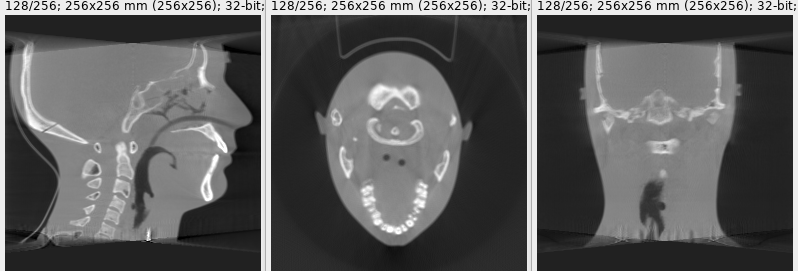
\includegraphics[width=0.8\textwidth]{reconstruction}
                    \caption{Ricostruzione del fantoccio presentato in \textit{Figura \ref{fig:skull-phantom}}, utilizzando la procedura \textit{rtkfdk}.}
                    \label{fig:reconstruction}
                \end{figure}
                
                L'immagine sinistra è una sezione del piano sagittale, l'immagine centrale è una sezione del piano coronale e l'immagine destra è una sezione del piano trasverso \cite{planes}.
                
            \bigskip
            \par
                E' possibile testare tutti gli altri algoritmi di ricostruzione all'interno della cartella \textit{RTK-bin/bin} senza dover rigenerare il file di geometria XML e lo Stack di proiezione MHA normalizzato. 
            
            
    \chapter{Creazione Package Python}
        \par
            Le procedure descritte da Sezione \ref{sec:lettura-csv} a Sezione \ref{sec:ricostruzione}, inizialmente implementate come script Python indipendenti, sono state riassemblate in moduli e collezionate in un unico Package. Il software è stato successivamente esteso presentando un'interfaccia utente testuale ed implementando un'architettura a directory per la lettura automatica delle informazioni. Infine, si è provveduto alla registrazione del Package all'interno del repository PyPI permettendo l'installazione del Package mediante il package manager PIP, disponibile di default a partire dalla versione 3.4 di Python.
            
        \section{Architettura}
            
        \section{Creazione Package}
        \section{Gestione Directory}
        \section{Interfaccia utente}
        \section{Registrazione su PyPI}
        \section{Estensione}
            
    \chapter{Risultati e Conclusioni}
        \section{Risultati}
        \section{Conclusioni}



\newpage
\begin{thebibliography}{1}
    
    \bibitem{hounsfield-nobel-lecture}
        Godfrey N. Hounsfield - Nobel Lecture, 8 December 1979.
    
    \bibitem{thomas-edison-brain}
        Shephard, D.A., Edison's attempts at radiography of the brain (1896), Mayo Clin. Proc., 1974.
    
    \bibitem{vallebona-pensiero}
        Vallebona A. - Gli ottanta anni della radiologia medica in Liguria. Atti dell’Accademia Ligure di Scienze e Lettere, XXXI: 18-46, 1974.
      
    \bibitem{vallebona-difesa}
        Vallebona A. - A proposito di un nuovo metodo radiografico chiamato "Planigrafia", Radiologia Medica Vol.XIX, fase 8, 1932-X.
    
    \bibitem{vallebona-ricordo}
        Franco Bistolfi, Alessandro Vallebona 1899-1987. Ricordo di un grande radiologo e del suo contributo allo sviluppo delle scienze radiologiche (PDF), in Fisica in Medicina, nº 2, 2005, pp. 115-123.  
    
    \bibitem{conventional-tomography}
        Littleton, J.T. "Conventional Tomography". A History of the Radiological Sciences (PDF). American Roentgen Ray Society. Retrieved 11 January 2014.
    
    \bibitem{nobel-debate}
        Riddle of the Nobel debate - Science 04 Jan 1980: Vol. 207, Issue 4426, pp. 37-38
    
    \bibitem{hounsfield-autobiografia}
        Les Prix Nobel. The Nobel Prizes 1979, Editor Wilhelm Odelberg, (Nobel Foundation), Stockholm, 1980. 
    
    \bibitem{scanner-story}
        Garry Pownall - The Scanner Story - Film, 1977.
    
    \bibitem{generazionale}
        Mahadevappa Mahesh. "Historical Developments." MDCT Physics: The Basics: Technology, Image Quality and Radiation Dose. 1st ed. N.p.: LWW, 2009.
    
    \bibitem{zeng}
        Gengsheng, Z. L. - Medical Image Reconstruction, a Conceptual Tutorial. In Springer (Ed.), 2010.
    
    \bibitem{mark-kac}
        \url{https://en.wikipedia.org/wiki/Hearing_the_shape_of_a_drum}
    
    \bibitem{history-radiology}
        Arpan K., Banerjee. "Chapter 6" The History of Radiology. By Adrian M. K. Oxford: OUP, 2013.
        
    \bibitem{lambert-beer}
        \url{https://en.wikipedia.org/wiki/Beer%E2%80%93Lambert_law}
        
    \bibitem{fessler}
        \url{http://web.eecs.umich.edu/~fessler/papers/files/talk/11/spie.pdf}    
        
    \bibitem{simplertk-wiki}
        \url{http://wiki.openrtk.org/index.php/SimpleRTK}
        
    \bibitem{swig-website}    
        \url{http://www.swig.org/}    
        
    \bibitem{cuda}
        \url{https://it.wikipedia.org/wiki/CUDA}
        
    \bibitem{rtk-classi}
        \url{http://www.openrtk.org/Doxygen/namespacertk.html}
        
    \bibitem{rtk-users-proj-offset}
        \url{http://public.kitware.com/pipermail/rtk-users/2014-December/000344.html}
    
    \bibitem{rtk-geometry}
        \url{http://www.openrtk.org/Doxygen/geometry.pdf}
        
    \bibitem{itk-doc}
        \url{https://itk.org/ItkSoftwareGuide.pdf}   
        
    \bibitem{voronoi}
        \url{https://en.wikipedia.org/wiki/Voronoi_diagram}
        
    \bibitem{delaunay}
        \url{https://en.wikipedia.org/wiki/Delaunay_triangulation}
    
    \bibitem{raw}
        \url{https://en.wikipedia.org/wiki/Raw_image_format}
    
    \bibitem{mha-doc}
        \url{https://itk.org/Wiki/ITK/MetaIO/Documentation} 
    
    \bibitem{endianness}
        \url{https://en.wikipedia.org/wiki/Endianness}


        
    \bibitem{script-bash}
        \url{https://github.com/dannylessio/auto-build-RTK}
    
    \bibitem{parallel-j}
        \url{https://www.gnu.org/software/make/manual/html_node/Parallel.html}    
    
    \bibitem{wiki-rtk}
        \url{wiki.openrtk.org}    
        
    \bibitem{simplertk-install}
        \url{http://wiki.openrtk.org/index.php/SimpleRTK}    
        
    \bibitem{python-pip}
        \url{https://pypi.python.org/pypi/pip}    
        
    \bibitem{simpleitk-install}
        \url{https://itk.org/Wiki/SimpleITK/GettingStarted}
        
    \bibitem{itk-image-object}
        \url{https://itk.org/SimpleITKDoxygen/html/classitk_1_1simple_1_1Image.html}
        
    \bibitem{sitk-write-image}
        \url{https://itk.org/SimpleITKDoxygen/html/classitk_1_1simple_1_1ImageFileWriter.html}
        
    \bibitem{pyexcel}
        \url{https://github.com/pyexcel/pyexcel}
        
    \bibitem{pyexcel-docs}
        \url{http://pyexcel.readthedocs.io/en/latest/generated/pyexcel.Sheet.html#pyexcel.Sheet}
        
    \bibitem{python-list}
        \url{https://docs.python.org/3/library/stdtypes.html#lists} 
       
    \bibitem{python-append}
        \url{https://docs.python.org/3/tutorial/datastructures.html#more-on-lists}
        
    \bibitem{sitk-image}
        \url{https://itk.org/SimpleITKDoxygen/html/classitk_1_1simple_1_1Image.html}
    
    \bibitem{python-range}
        \url{https://docs.python.org/3/library/stdtypes.html#range}
        
    \bibitem{python-iterable}
        \url{http://stackoverflow.com/questions/9884132/what-exactly-are-pythons-iterator-iterable-and-iteration-protocols} 
        
    \bibitem{sitk-estractor}
        \url{https://itk.org/SimpleITKDoxygen/html/classitk_1_1simple_1_1ExtractImageFilter.html#details}
        
    \bibitem{sitk-log}
        \url{https://itk.org/SimpleITKDoxygen/html/classitk_1_1simple_1_1LogImageFilter.html#details}
        
    \bibitem{python-floating-point}
        \url{https://docs.python.org/3/library/functions.html#float}
    
    \bibitem{sitk-star-operator}
        \url{https://itk.org/SimpleITKDoxygen/html/sitkImageOperators_8h_source.html#l00050}
    
    \bibitem{sitk-joinseries}
        \url{https://itk.org/SimpleITKDoxygen/html/classitk_1_1simple_1_1JoinSeriesImageFilter.html#details}
    
    \bibitem{sitk-copy-information}
        \url{https://itk.org/SimpleITKDoxygen/html/classitk_1_1simple_1_1Image.html#afa8a4757400c414e809d1767ee616bd0}

    \bibitem{input-python}
        \url{https://docs.python.org/3/library/functions.html#input}
        
    \bibitem{rtk-recon-list}
        \url{http://www.openrtk.org/Doxygen/files.html}
    
    \bibitem{imagej}
        \url{https://imagej.nih.gov/ij/}
        
    \bibitem{imagej-3dio-plugin}
        \url{http://ij-plugins.sourceforge.net/plugins/3d-io/index.html}
        
    \bibitem{planes}
        \url{https://it.wikipedia.org/wiki/Posizione_anatomica}

    \end{thebibliography}
\end{document}
